\documentclass{ludis} % pieejams https://github.com/rihardsk/LU-nosl-guma-darbs---LaTeX

% xelatex
\usepackage{fontspec}
\usepackage{xunicode}
\usepackage{xltxtra}

%\usepackage[utf8]{inputenc}

\usepackage[]{hyperref}
\hypersetup{
    colorlinks=false
}
\urlstyle{same}

% languages
\usepackage{fixlatvian}
\usepackage{polyglossia}
\setdefaultlanguage{latvian}
\setotherlanguages{english,russian}

% fonts
\usepackage{xltxtra}
% \setmainfont[Mapping=tex-text]{Times New Roman}
%\defaultfontfeatures{Scale=MatchLowercase,Mapping=tex-text}

% bibliography
%\usepackage{csquotes}
\usepackage[
    backend=biber,
    style=numeric-comp,
    sorting=none,
    natbib=true,
    url=false,
    doi=true%,
    %eprint=false
]{biblatex}
\addbibresource{bibliography.bib}

% toc
\setcounter{secnumdepth}{3}
\setcounter{tocdepth}{3}

%tables
\usepackage{longtable}

%papildus matemātika
\usepackage[showonlyrefs]{mathtools}
\newenvironment{thmenum}
 {\begin{enumerate}[label=\upshape(\arabic*),ref=\thethm(\arabic*)]}
 {\end{enumerate}}
\usepackage{amsmath}

%pseidokodam
%\usepackage[noend]{algpseudocode}
%\usepackage{algpseudocode}
\usepackage[boxed,linesnumbered]{algorithm2e}
\SetAlgorithmName{Algoritms}{}{Algoritmu saraksts}

%main line spacing, kur vajag
\usepackage{setspace}

%lai flushotu floatus
\usepackage{placeins}

%images
\usepackage{graphicx}
\usepackage{float}
\usepackage{svg}

%dalīšana kolonnās
\usepackage{multicol}

%saraksti
\usepackage{enumitem}

\fakultate{Datorikas}
\nosaukums{Paredzošā stimulētā mācišanās}
\darbaveids{Maģistra kursa}
\autors{Rihards Krišlauks}
\studapl{rk09006}
\vaditajs{Asoc.prof., Dr. dat. Jānis Zuters}
%\recenzents{Juris Vīksna profesors Dr.sc.comp.}
\vieta{Rīga}
\gads{2015}

\begin{document}
\maketitle

\begin{abstract-lv}
  TODO

\keywords{stimulētā mācīšanās; neironu tīkli; Markova izvēles procesi; nepārtrauktas telpas.}
\end{abstract-lv}
\clearpage

\begin{abstract-en}
  TODO

\keywords{reinforcement learning; artificial neural networks; Markov decision processes; continuous spaces.}
\end{abstract-en}


\tableofcontents

\iffalse
\specnodala{Apzīmējumu saraksts}
\setlength\LTleft{0pt}
\setlength\LTright{0pt}
\begin{longtable}{| c | p{28em} |}
  \hline
  \textbf{Apzīmējums} & \textbf{Atšifrējums}\\ 
  \endhead

  \hline
  $D_X \in \mathbb{N}_+$ & \\ %TODO šis jādefinē arī telpas elementiem
  $S \subseteq \mathbb{R}^{D_S}$ & \\
  $A \subseteq \mathbb{R}^{D_A}$ & \\
  $R:S \times A \times S \rightarrow \mathbb{R}$ & \\
  $T:S \times A \times S \rightarrow [0,1]$ & Apzīmējuma nosaukums \\
  $\pi(s, a)$ &  Apzīmējuma nosaukums 2\\
  \hline
\end{longtable}
\fi

\specnodala{Ievads}
Pēdējā laikā teorētiskajā neirozinātnē plašu piekrišanu sāk iegūt t.s.
paredzošās kodēšanas (predictive coding) teorija, kuras pamattēze ir --
smadzenes ir paredzēšanas mašīnas, tās pastāvīgi cenšas sapārot ienākošos
sensoru signālus ar augsta līmeņa paredzējumiem ar mērķi minimizēt paredzēšanas
kļūdas. Paredzošā kodēšana sniedz vienotu skatījumu uz procesiem, kas ir pamatā
cilvēka apziņai, un piedāvā mehānismu, kas ļauj izskaidrot plašu klāstu ar
neirozinātnē pētītiem cilvēka apziņas fenomeniem \autocite{Clark2013}.

Ideja par smadzenēm kā māšīnām, kas, ņemot vērā pašreizējos novērojumus, cenšas
paredzēt nākotnes novērojumus, ir ļoti pievilcīga no dažādu mašīnmācīšanās
paradigmu skatpunkta. Šis vienkāršais mehānisms šķiet viegli formulējams kā
mašīnmācīšanās problēma, un šķiet it īpaši piemērots, lai to izteiktu kā
stimulētās mācīšanās problēmu.

Stimulētā mācīšanās ir mašīnmācīšanās paradigma, kas formalizē mācīšanos kā
mašīnmācīšanās uzdevumu. Tās pamatā ir ideja par vidi un aģentu, kas tajā
darbojas. Aģenta mērķis ir, ņemot vērā ārēju atalgojuma signālu, veikt darbības
vidē tā, lai maksimizētu saņemto atalgojumu. Šis vienkāršais, bet spēcīgais,
uzstādījums ļauj aprakstīt un risināt ļoti plašu problēmu loku, kur optimālā
rīcības stratēģija nav zināma, bet ir iespējams nodefinēt stāvokli, ko aģentam
būtu jācešas sasniegt. Aģenta ziņā paliek, darbojoties vidē, laika gaitā atrast
optimālo stratēģiju, kas ļautu sasniegt pēc iespējas lielāku atalgojumu. Kā
piemērus šādi risināmām problēmām var minēt orientēšanos labirintā vai
automātisku lidaparāta kontroli.

No augstāk minētā dabīgi seko doma par paredzošās kodēšanas ideju pielietošanu
stimulētās mācīšanās uzdevumu risināšanā. Interesi raisa ideja par vides nākamā
stāvokļa paredzēšanu, ņēmot vērā pašreizējo, un vai tas palīdzētu mācīšanās
procesā. Tas liktu stimulētās mācīšanās aģentam tuvināti iemācīties vides
modeli. Tuvākas izpētes vērts ir jautājums, vai šāds iekšējs modelis palīdzētu
macīšanās procesā.

Šajā darbā tiks pētītas iespējas, izmantot paredzošās kodēšanas idejas stimulētās
mācīšanas uzdevumu risināšanai, kā arī tiek pētītas dažādas citas iespējas ar
papildus informāciju uzlabot mācīšanās ātrumu. Darbs tiek iesākts ar vispārīgu stimulētās
mācīšanās paradigmas apskatu, kur autors galvenokārt pieturas pie izklāsta kas
atrodams \autocite{Krislauks2015}. Tam seko COMBO CACLA algoritma apraksts, un
salīdzinājums ar CACLA algoritmu, uz kā tas ir balstīts. %TODO papildināt, kad
                                %ir vairāk gatavs no satura
%NOTE: pie cacla algoritma jāpastāsta, kas ir tie aspekti, kas padara viņu
%pievilcīgu modifikācijām.

\chapter{Markova izvēles procesi} \label{chap:mdp}
Nodaļā tiek apskatīti Markova izvēles procesi ar mērķi sniegt vispārīgu
priekšstatu par tēmu. Tiek doti arī piemēri un paņēmieni, kas tieši neattiecas
uz darba mērķi, bet doti, lai vieglāk izprast jēdziena kontekstu, tomēr lielākā
daļa izklāsta ir pozicionēta tieši vēlāk apskatāmās stimulētās mācīšanās
kontekstā.

Markova izvēles procesi (angliski \textit{Markov decision processes}, turpmāk
tekstā - MDP) formalizē un ļauj modelēt izvēles veikšanas procesu apstākļos, kur
darbības rezultāts ir atkarīgs tikai no sistēmas pašreizējā stāvokļa, bet ir
daļēji nejaušs, t.i., izvēles veicējs procesu kontrolē tikai daļēji. Mērķis ir
kontrolēt sistēmu tā, lai tiktu maksimizēta kāda metrika, kas ir atkarīga no
katrā solī veiktās darbības rezultāta. Tiek uzskatīts, ka MDP ir ieviesti
\autocite{Bel}.

MDP vispārina MI (mākslīgā intelekta) plānošanas paradigmu
\autocite{Hendler1990ai}. Tie ļauj plānošanas problēmu modelī iekļaut nejaušību,
kas saistīta ar darbību izpildi, un ļauj specificēt mazāk konkrētus plāna
mērķus. Turklāt MDP ļauj formalizēt sistēmas, kuru darbībā jāņem vērā resursu
patēriņš. Plāns MI plānošanas izpratnē kā soļu virkne, kas paredzēta, lai no
sākuma stāvokļa sasniegtu uzdoto beigu stāvokli, MDP formālismā tiek vispārināts
par stratēģiju, jeb funkciju, kas katram sistēmas stāvoklim piekārto optimālo
darbību, tā lai sistēmas kontroles procesā tiktu maksimizēta kāda no uzdevuma
atkarīga metrika.

\autocite{Otterlo} tiek dots piemērs tipiskai MI plānošanas problēmai. Var
iedomāties, ka ir dota kāda telpa ar tajā sakrāmētām kastēm, un uzdevums ir
kastes pārkrāmēt tā, lai dažas no tām pārliktu norādītās vietās. Šo uzdevumu var
risināt ar MI plānošanas metodēm. Toties, ja tiek apskatīta situācija, kur kastu
krāmēšanas operators, piemēram, robots, darbības neizpilda pilnīgi precīzi, bet
var pieļaut kļūdas, vai arī var iestāties kādi citi apstākļi, kas nav operatora
kontrolē, tad šādam uzstādījumam dabīgāk atbilst MDP paradigma, kurā var,
teiksim, uzdevuma mērķi atslābināt un teikt, ka uzdevuma mērķis ir maksimizēt
atalgojumu, kas saņemts par katras kastes nolikšanu vietā.

Pieeju MDP risināšanai vada par sistēmu pieejamās informācijas veids. Gadījumus,
kad par sistēmu pieejamā informācija ir pilnīga, t.i., ir zināma sistēmas
stāvokļu pāreju dinamika, kā arī ar darbību veikšanu saistītā atalgojumu
funkcija, parasti mēdz risināt ar dinamiskās programmēšanas metodēm. Savukārt,
grūtāko uzstādījumu, kur par sistēmu nav zināma nekāda sākotnējā informācija, un
informācija par sistēmas pārejām un atalgojumiem ir noskaidrojama tikai ar to
mijiedarbojoties, risina ar stimulētās mācīšanās metodēm, kas tiek apskatītas
šajā darbā.

Tālāk tiek ieviesta Markova izvēles procesu definīcija. Mēs lietosim definīciju,
kas pieļauj nepārtrauktas stāvokļu un darbību telpas. Ievērosim, ka definīciju
var sašaurināt uz diskrētām stāvokļu vai darbību telpām, ņemot $S \subseteq
\mathbb{N}^{D_S}$ vai $A \subseteq \mathbb{N}^{D_A}$.

\begin{definicija}
Par Markova izvēles procesu, jeb MDP, sauc kortežu $(S, A, T, R)$, kur:
\begin{itemize}
	\item $S \subseteq \mathbb{R}^{D_S}$, kur $D_S \in \mathbb{N}$, ir stāvokļu
    kopa, %TODO iespējams bezgalīga?
	\item $A \subseteq \mathbb{R}^{D_A}$, kur $D_A \in \mathbb{N}$, ir darbību
    kopa, %TODO iespējams bezgalīga?
	\item $T:S \times A \times S \rightarrow [0,1]$ ir pārejas funkcija, kur $T(s,
    a, s')$ norāda varbūtību, esot stāvoklī $s \in S$ veicot darbību $a \in A$,
    nonākt stāvoklī $s' \in S$,
	\item $R:S \times A \times S \rightarrow \mathbb{R}$ ir atalgojuma funkcija,
    $R(s, a, s')$ norāda atalgojumu, kas tiek saņemts, esot stāvoklī $s \in S$
    veicot darbību $a \in A$ un pēc tam nonākot stāvoklī $s' \in S$.
\end{itemize}
Ja stāvokļu telpa ir nepārtraukta, $T(s, a, s')$ apzīmē varbūtību blīvuma
funkciju, jeb
\[
	\int_{S'} T(s, a, s')ds' = P(s_{t+1} \in S' \mid s_t = s \land a_t = a),
\]
kas norāda varbūtību, ka stāvoklī $s \in S$, veicot darbību $a \in A$ pāreja
beigsies stāvoklī, kas pieder apgabalam $S'$. %TODO jāpaskaidro _t un _{t+1}?
\end{definicija}
%TODO beigu stāvokļi?

MDP definīcijā mēdz arī iekļaut atlaides koeficientu (angliski \textit{discount
  factor}), ko apzīmē ar $\gamma \in [0,1]$. Tas raksturo to, kā atšķiras
nākotnē saņemtie no tagadnē saņemtajiem atalgojumiem. Šajā darbā tiek pieņemts,
ka $\gamma$ pieder pie katra konkrētā algoritma specifikācijas. %TODO šis vārds
                                %izbīdāš aiz paragrāfa malas robežas
Tas tiek darīts tādēļ, ka $\gamma$ divi dažādi algoritmi vienā un tajā pašā
uzdevumā var sniegt dažādus rezultātus pie dažādām $\gamma$ vērtībām, %TODO
                                %vajag atsauci
tāpēc $\gamma$ izvēle tiek atstāta algoritma ziņā, tā kā tā maiņā neietekmē
uzdevuma būtību. %TODO ok, šīs varbūt ir muļķības. ko darīt, ja gamma ir
                 %līdzeklis, ar ko specificēt kādu uzdevumam noderīgu aspektu?
Šādā veidā MDP tiek ieviesti arī \autocite{Otterlo}.

Parasti tiek ieviesta arī funkcija $\pi: S \times A \rightarrow [0, 1]$, kas
apzīmē optimālo stratēģiju, jeb kontroles shēmu:
\[
	\pi(s, a) = P(a_t = a \mid s_t = s),
\]
kur $\sum_{a\in A} \pi(s,a)=1$, ja darbību telpa ir diskrēta, un $\int_{A}
\pi(s,a) da = 1$, ja tā ir nepārtraukta. Funkcija norāda varbūtību, ar kādu
optimālajā stratēģijā esot stāvoklī $s \in S$ tiek veikta darbība $a \in A$.
Gadījumā, ja darbību telpa ir nepārtraukta, $\pi$ ir varbūtību blīvuma funkcija.

Neformāli to var iedomāties (no stimulētās mācīšanās pieejas skatpunkta) kā
procesu, kur darbību veicējs, sauksim viņu par aģentu, var novērot to, kādā
stāvoklī sistēma ir pašlaik, un viņam ir pieejama informācija par darbībām, ko
ir iespējams veikt. Aģents izvēlas darbību un novēro jauno stāvokli, uz kuru
pāriet sistēma, kā arī rezultātā saņemto atalgojumu. Aģenta mērķis ir izvēlēties
darbības tā, lai maksimizētu laika gaitā saņemto atalgojumu. Aģents iepriekš
nezina ne varbūtību, ar kādu tiks veikta viņa izvēlētā pāreja, ne pašu stāvokli,
uz kuru pāries sistēma, ne arī atalgojumu, ko saņems. Šo informāciju viņam ir
jāuzkrāj laika gaitā no iepriekšējās pieredzes.

Jāņem vērā, ka uzdevumu sarežģī tieši iepriekš minētā nenoteiktība. Sākot darbu,
aģentam iepriekš nezināmā domēnā, tam trūkst jebkādas informācijas par uzdevumu,
un tā ir iegūstama tikai mijiedarbojoties ar domēnu. Turklāt par izdarītās
izvēles labumu liecina nevis uzreiz pēc tās veikšanas saņemtais atalgojums, bet
gan arī atalgojums, kas saņemts nākotnē, pēc šī stāvokļa apmeklēšanas. Citiem
vārdiem -- darbības izdevīgums ir jāvērtē ilgtermiņā. Vēl viens aspekts, kura
nozīme pieaug jo īpaši nepārtrauktās stāvokļu un darbību telpās, ir soļu skaits,
pēc kura aģents atrod stratēģiju, kas tuva optimālajai. Ja pārtrauktās, galīgās
stāvokļu telpās vēlme ir, lai, meklējot optimālo stratēģiju katrs stāvoklis
tiktu apmeklēts pēc iespējas mazāk reižu, tad nepārtrauktās stāvokļu un darbību
telpās katru stāvokli un darbību nemaz nav iespējams izmēģināt, tā kā to skaits
ir neierobežots. Šis apsvērums nošķir stratēģijas, kas izmantojamas MDP
risināšanas algoritmā. %TODO laikam slikti skan. jāpārformulē

%TODO jāievieš stāvokļu-darbību vērtības funkcija

%TODO jāievieš stāvokļu vērtības funkcija

%TODO jāpasaka, kas ir Belmana vienādojumi, varbūt

Jāpiebilst, ka tie paši apsvērumi, kas šajā nodaļā ir izteikti par nepārtrauktām
stāvokļu un darbību telpām, lielā mērā ir attiecināmi arī uz diskrētām, bet
lielām telpām. Turpmākajā tekstā, runājot par diskrētām telpām, domātas ir
telpas, kuras ir pietiekami mazas. Konkrēti apmēri šeit netiek minēti, jo tie
atkarīgi no pieejamajiem skaitļošanas resursiem.

\section{Stratēģijas optimalitāte}
Darbā jau vairākkārt ir pieminēts, ka stratēģijai, kas tiek izmantota MDP
kontrolē jāapmierina kaut kādus optimalitātes kritērijus. Izteiksim šo prasību
formālāk, norādot trīs iespējamos optimalitātes kritērijus, kā tie ieviesti
\autocite{Otterlo}.

\begin{definicija}
Teiksim, ka dotam MDP, ko apzīmēsim ar $M$, stratēģija $\pi$ ir optimāla galīgā
horizonta nozīmē, ja tā maksimizē izteiksmi:
\[
	E\left[\sum_{t=0}^{h}r_t\right],
\]
kur $h \in \mathbb{N}$ ir horizonta izmērs, un $r_t$ apzīmē $t$-ajā solī saņemto
atalgojumu, kontrolējot $K$ pēc shēmas $\pi$.
\end{definicija}

\begin{definicija}
Teiksim, ka dotam MDP, ko apzīmēsim ar $M$, stratēģija $\pi$ ir optimāla
bezgalīgā horizonta nozīmē, ja tā maksimizē izteiksmi:
\[
	E\left[\sum_{t=0}^{\infty}\gamma^t r_t\right],
\]
kur $\gamma \in \left[0, 1\right)$ ir atlaides koeficients, un $r_t$ apzīmē
$t$-ajā solī saņemto atalgojumu, kontrolējot $K$ pēc shēmas $\pi$.
\end{definicija}

\begin{definicija}
Teiksim, ka dotam MDP, ko apzīmēsim ar $M$, stratēģija $\pi$ ir optimāla vidējā
atalgojuma nozīmē, ja tā maksimizē izteiksmi:
\[
	\lim\limits_{h \rightarrow \infty} E\left[\frac{1}{h}\sum_{t=0}^{h}r_t\right],
\]
kur $h \in \mathbb{N}$ ir horizonta izmērs, un $r_t$ apzīmē $t$-ajā solī saņemto
atalgojumu, kontrolējot $K$ pēc shēmas $\pi$.
\end{definicija}

Optimalitātes kritērija izvēle var būt atkarīga no risināmās problēmas. Pārskats
par dažādu optimalitātes kritēriju izmantošanu MDP modelēšanā ir dots
\autocite{koenig2002interaction}. Turpmāk tekstā tiks izmantots bezgalīgā
horizonta optimalitātes nosacījums.

%TODO svarīgi, pārskata grāmata saka, ka kritērijus ar konkrētu \pi sasaista
%value funkcija. es savukārt neredzu iemeslu, kāpēc mest \pi no definīcijas
%laukā

\section{Vērtības funkcija un stāvokļu-darbību vērtības funkcija}
Stāvokļu vērtības funkcija, vai vienkāršāk -- vērtības funkcija -- tiek
ieviesta, lai izteiktu stāvokļa vērtību pie konkrētas stratēģijas. Tā izsaka,
cik izdevīgi ir atrasties kādā stāvoklī pie dotās stratēģijas, ņemot vērā
optimalitātes nosacījumu.
\begin{definicija}
Teiksim, ka ir dota kontroles shēma $\pi$. Tai atbilstošā stāvokļu vērtības
funkcija $V^\pi : S \rightarrow \mathbb{R}$ izsaka sagaidāmo atalgojumu, sekojot
stratēģijai $\pi$, sākot no stāvokļa $s$:
\begin{equation} \label{eq:vpi}
	V^\pi (s) = E_\pi \left\{ \sum_{k=0}^{\infty} \gamma^k r_{t+k} \mid s_t = s\right\}
\end{equation}
\end{definicija}

Līdzīgi var ieviest arī stāvokļu-darbību vērtību funkciju:
\begin{definicija}
Teiksim, ka ir dota kontroles shēma $\pi$.
Tai atbilstošā stāvokļu-darbību vērtības funkcija $Q^\pi : S \times A
\rightarrow \mathbb{R}$ izsaka sagaidāmo atalgojumu, sekojot stratēģijai $\pi$,
sākot no stāvokļa $s$ un veicot darbību $a$:
\[
	Q^\pi (s,a) = E_\pi \left\{ \sum_{k=0}^{\infty} \gamma^k r_{t+k} \mid s_t = s \land a_t = a\right\}
\]
\end{definicija}

Tagad varam pārformulēt optimālās stratēģijas jēdzienu:
\begin{definicija}
Teiksim, ka stratēģija ir optimāla, un apzīmēsim to ar $\pi^*$, ja visiem
stāvokļiem $s \in S$ un visām stratēģijām $\pi$ izpildās:
\[
	V^{\pi^*}(s) \geq V^{\pi}(s)
\]
\end{definicija}

\section{MDP risināšana un Bellmana vienādojumi}
Īsumā ieskatīsimies MDP risināšanas iespējās. Bellmana optimalitātes vienādojums
ļauj rekursīvi izteikt optimālo stāvokļu vērtības funkciju $V^* = V^{\pi^*}$
atkarībā no pārejas un atalgojuma funkcijām
\autocite{Bel}\autocite{Otterlo}\autocite{Hasselt2012}. Šeit tas ir izteikts
nepārtrauktām stāvokļu telpām: 
\[
	V^*(s) = \max_{a\in A} \int_S T(s,a,s')\left(R(s,a,s') + \gamma V^*(s)\right) ds'.
\]
Vienādojums sniedz arī veidu, kā izteikt pašu optimālo stratēģiju:
\begin{equation}
	\pi^*(s) =  \arg \max_{a} \int_S T(s,a,s')\left(R(s,a,s') + \gamma V^*(s)\right) ds'. \label{eq:1}
\end{equation}
Līdzīga sakarība ir arī spēkā optimālajai stāvokļu-darbību vērtības funkcijai $Q^* = Q^{\pi^*}$:
\[
	Q^*(s, a) = \int_S T(s,a,s')\left(R(s,a,s') + \gamma \max_{a'}Q^*(s',a')\right) ds'.
\]
$Q^*$ un $V^*$ saista sakarības:
\[
	Q^*(s, a) = \int_S T(s,a,s')\left(R(s,a,s') + \gamma V^*(s')\right) ds',
\]
\[
	V^*(s) = \max_{a} Q^*(s,a),
\]
kas ļauj izteikt optimālo stratēģiju arī ar stāvokļu-darbību vērtības funkciju:
\begin{equation}
	\pi^*(s) = \arg \max_a Q^*(s, a). \label{eq:2}
\end{equation}

Augstāk redzamie vienādojumi ļauj kategorizēt veidus, kādos risināmi MDP.

\subsection{Modeļa aproksimācija}
Modeļa aproksimācijas pieejā tiek mēģināts tuvināti atrast dotās MDP nezināmos
parametrus -- pāreju funkciju $T$ un atalgojuma funkciju $R$ --, lai no tām
atvasinātu aproksimētās MDP optimālo kontroles shēmu. Modeļa meklēšanā tiek
pieņemts, ka kopas $S$ un $A$ ir zināmas. Dziļākam ieskatam metodēs, kas tiek
izmantotas modeļa aproksimēšanā, skatīt \autocite{nguyen2011model}.

Kad modelis ir zināms, optimālās stratēģijas atrašana galīgam stāvokļu un
darbību telpām ir samērā vienkārša. Var tikt izmantots, piemēram, \textit{value
  iteration} vai \textit{policy iteration} algoritms, kam ir var pierādīt, ka
tie konverģē uz optimālo $\pi^*$ \autocite{Barto}. Tomēr vispārīgā gadījumā MDP
nepārtrauktās stāvokļu telpās situācija ir krietni sarežģītāka -- katram katram
stāvoklim optimālo stratēģiju atrast nav iespējams \autocite{Otterlo}. Piemēram,
iepriekš minētie \textit{value iteration} un \textit{policy} iteration algoritmi
satur ciklu pa visu stāvokļu kopu, kas algoritmu padara nelietojamu, ja stāvokļu
skaits ir bezgalīgi liels.

%TODO šo varbūt var iekļaut: Alternatīvi \autocite{Otterlo} tiek minēta iespēja
%tuvināto MDP izmantot, lai ģenerētu 

Lai arī iepriekš minētie argumenti nav spēkā uz MDP ar nepārtrauktām darbību
telpām, autors neredz tiešu veidu, kā pieeja būtu vispārināma, lai no iegūtā MDP
modeļa atvasinātu stratēģiju, kas optimālo darbību stāvoklī atrod ar neirona
tīkla palīdzību.
%TODO jāpasaka, kāpēc neironu tīkls būtu labāks
Turklāt, lai arī kā darba mērķis netika uzstādīta prasība algoritmam darboties
arī ar nepārtrauktām stāvokļu telpām, nevajadzīga algoritma vispārīguma
samazināšana, ja no tā var izvairīties, tiek uzskatīta par nevēlamu.

Vēl ir jāmin, ka metodes aproksimētā modeļa risināšanai ir tuvākas dinamiskās
programmēšanas paradigmai, tāpēc tās šķiet mazāk saistošas. Pastāv gan arī
hibrīd varianti, kur modelis tiek aproksimēts, lai uz tā veiktu trenēšanu ar
stimulētās mācīšanās metodēm, gadījumos, kad mācīšanās īstajā domēnā ir pārāk
resursietilpīga, bet šīs metodes saskaras jau ar citām problēmām
\autocite{Hasselt2012}.

\subsection{Vērtību aproksimācija}
Vērtību aproksimācijas piegājienā tiek nevis mēģināts atrast trūkstošās pāreju
un atalgojuma funkcijas, bet gan tiek uzreiz mēģināts tuvināti atrast funkcijas
$V^*$ vai $Q^*$. Kā redzams iepriekšējā sadaļā, vienādojumi \eqref{eq:1} un
\eqref{eq:2} ļauj atrast $\pi^*$, ja $V^*$ vai $Q^*$ ir zināma. Šīs kategorijas
algoritmus iedala atkarībā no tā, vai tie ir spējīgi mācīties tiešsaistē, un vai
algoritms ir \textit{on-policy} vai \textit{off-policy} tipa.

Atsaucoties uz \autocite{Hasselt2012} -- \textit{on-policy} algoritmi mēģina
tuvināti atrast stāvokļu vērtības funkciju $V^\pi$ vai stāvokļu-darbību vērtības
funkciju $Q^\pi$ stratēģijai $\pi$, kura konkrētajā brīdī tiek izmantota. Lai
arī optimālā stratēģija $\pi^*$ iesākumā nav zināma, \textit{on-policy}
algoritmi pakāpeniski nonāk pie optimālās funkcijas $V^{\pi^*}$ vai $Q^{\pi^*}$,
iteratīvi katrā solī uzlabojot sev zināmo $\pi$. \textit{Off-policy} tipa
algoritmi izmanto citu pieeju, kas tiešā veidā necenšas atrast optimālo
stratēģiju $\pi^*$. Funkciju $V^{\pi^*}$ vai $Q^{\pi^*}$ novērtējumi var tikt
uzlaboti, sekojot stratēģijām, kas nav optimālas.

Algoritmus, kas spējīgi mācīties tiešsaistē, jeb \textit{online} algoritmus,
raksturo tas, ka tie savus novērtējumus pielāgo pēc katras pārejas veikšanas,
novērojot jauno sistēmas stāvokli un saņemto atalgojumu. Pretnostatījumā
\textit{offline} algoritmi ieejas datus apstrādā pa vairākiem novērojumiem vienā
grupā. \textit{Online} algoritmiem ir raksturīgas mazākas prasības pēc
skaitļošanas resursiem viena novērojuma apstrādāšanai. Tie strādā labi
gadījumos, kad novērojumu ir pieejams daudz un viena novērojuma veikšana nav
resursietilpīga. \textit{Offline} algoritmi savukārt efektīvāk izmanto pieejamos
novērojumus, kas tiem ļauj līdzvērtīgu rezultātu sasniegt, apstrādājot mazāk
novērojumu.

Pie \textit{on-policy} algoritmiem pieder, piemēram,
\textit{temporal-difference} saimes algoritmi. Pie \textit{off-policy}
algoritmiem pieskaitāms, piemēram, ir \textit{Q-learning} un tā varianti. Katrā
minēto algoritmu grupā ietilpst gan \textit{online}, gan \textit{offline}
algoritmu varianti \autocite{Barto}.

Minētajiem algoritmiem darbošanās nepārtrauktās stāvokļu telpās nesagādā
problēmas. Šādās situācijās parasti $V^{\pi^*}$ vai $Q^{\pi^*}$ reprezentācijai
tiek izmantota kāda funkciju aproksimēšanas pieeja, piemēram, neironu tīkli. Kā
piemēru var skatīt \autocite{tesauro1995temporal}, kur neironu tīkls tiek
trenēts ar \textit{Q-learning}, lai aproksimētu funkcijas $Q^{\pi^*}$ vērtību
backgammon spēlē. Jaunākā avotā \autocite{mnih2013playing} \textit{Q-learning}
variants tiek izmantots, lai autonomi apmācītu aģentu spēlēt vairākas Atari 2600
videospēles, kā ieejas datus izmantojot tikai spēlēs ekrāna pikseļu vērtības
(bez īpašas priekšapstrādes) un spēles rezultātu. $Q^{\pi^*}$ aproksimēšanai
tiek izmantots neironu tīkls. Šis rezultāts ir īpaši interesants, jo spēles
stāvokļu telpa ir izteikti sarežģīta, lai no spēles ekrāna pikseļu vērtībām būtu
iespējams kaut ko pateikt par pašreizējo spēles stāvokli, aģentam ir jāiemācās
pikseļu vērtības abstrahēt sarežģītākos objektos. To šeit paveic neironu tīkls.

Ar nepārtrauktām darbību telpām ir citādi. Tā kā bieži šajos algoritmos, lai
atrastu optimālo stratēģiju, atbilstoši \eqref{eq:2} tiek meklēts atrisinājums
izteiksmei
\[
	\arg \max_a Q^*(s, a),
\]
tad nevar iztikt bez darbību telpas diskretizēšanas. Literatūrā un praksē
sastopami dažādi diskretizācijas varianti -- sākot no vienkāršākajiem kā
\textit{tile coding}, kur darbību telpa tiek sadalīta nepārklājošos apgabalos,
kas katrs uztverams kā diskretizētās darbību telpas atsevišķs elements, līdz
sarežģītākām, kā, piemēram, \textit{Kanerva coding} \autocite{Barto}.

Algoritmus, kuros optimālā stratēģija tiek atvasināta no $Q^*$ funkcijas, kā
redzams augstāk, grūti vispārināt atbilstoši darba mērķim darbībai ar neironu
tīkliem, jo tas prasa algoritmam glabāt neironu tīkla vai kāda cita funkciju
aproksimētāja svarus, un tos darbības laikā pielāgot. Cik autoram zināms, šādas
problēmas pastāv \textit{off-policy} algoritmos, piemēram, minētajā
\textit{Q-learning}. \textit{On-policy} algoritmi šajā aspektā darba ietvaros
nav pētīti.

\subsection{Stratēģijas aproksimācija}
Atšķirībā no vērtību aproksimācijas algoritmiem, stratēģijas aproksimācijas
pieejas algoritmi optimālās stratēģijas tuvinājumu glabā tiešā veidā. Parasti
nav nekādu šķēršļu $\pi^*$ reprezentācijai izmantot kādu vispārīgu funkciju
aproksimētāju. Tādā gadījumā algoritms glabā tā parametrus. Šim nolūkam var tikt
izmantots arī neironu tīkls. Bez tuvinātas optimālās stratēģijas mēdz tikt
glabāta arī $V^{\pi^*}$ vai $Q^{\pi^*}$ funkcija. Algoritmus, kuros tiek tā
darīts, mēdz saukt par \textit{actor-critic} algoritmiem, ar vārdu
\textit{critic} atsaucoties uz algoritma daļu, kas vērtē spēles stāvokļa
izdevību, jeb $V^{\pi^*}$ vai $Q^{\pi^*}$, un ar \textit{actor} atsaucoties uz
stratēģiju. Pēc analoģijas, stratēģijas aproksimācijas algoritmus, kas neizmanto
kādu no vērtību funkcijām, dēvē par \textit{actor-only} algoritmiem, savukārt
vērtību aproksimācijas algoritmus -- par \textit{critic-only} algoritmiem.
Stratēģijas aproksimācijas algoritmi tiks tuvāk apskatīti \ref{chap:stim}
nodaļā.

\chapter{Funkciju aproksimācija}
Nodaļā tiks apskatītas funkciju aproksimācijas metodes, kas ir pamatā darbā
minētajiem stimulētās mācīšanās algoritmiem. Izklāsts ir daļēji tehniskas dabas,
bet tiek skaidrotas arī pielietojamo metožu sekas attiecībā uz stimulētās
mācīšanās uzdevumu veikšanu nepārtrauktās darbību telpās. Tiek likts uzsvars uz
nelineāro funkciju aproksimētāju, it īpaši neironu tīklu, apskatu, kā arī tiek
sniegta motivācija to lietojumam no tehniskās puses.
%Tiek arī apskatīti un īsumā izvērtēti citu klašu funkciju aproksimētāji. %,
%uzmanību pievēršot, piemēram, ģenētiskajiem algoritmiem.

Ar funkciju aproksimēšanu, sauktu arī par funkciju tuvināšanu, tiek saprastas
pieejas, kuru mērķis ir, par izejas datiem ņemot aproksimējamās, jeb mērķa,
funkcijas vērtības, atrast citu funkciju noteiktā klasē, kas pēc iespējas vairāk
atbilst aproksimējamajai. Bieži vien aproksimējamā funkcija kā tāda nemaz
nepastāv, bet aproksimēšana notiek ar mērķi iegūt funkciju, kas izsaka
sakarības, kas novērojamas kādā mūs interesējošā procesā. Skatoties
mašīnmācīšanās kontekstā, vai konkrētāk -- apskatot pārraudzītās mācīšanās
(\textit{supervised learning}) problēmu -- mērķis ir no dota datu korpusa, kas
satur kāda mūs interesējoša objekta parametrus, kam attiecināta kāda no
parametriem (iespējams daļēji) atkarīga vērtība, konstruēt funkciju, kas, ieejā
saņemot minētā veida parametrus, būtu spējīga prognozēt iepriekš neredzētu datu
punktu vērtības.

Stimulētās mācīšanās uzdevumos, kur tiek lietotas vērtību aproksimācijas
pieejas, funkciju aproksimēšana tiek lietota, lai ar kādiem domēnu aprakstošiem
parametriem izteiktu stāvokļu vai stāvokļu-darbību vērtību funkciju. Stratēģijas
aproksimācijas pieejās funkciju aproksimācija var tikt lietota, lai izteiktu
optimālo stratēģiju atkarībā no MDP stāvokļa. Funkciju aproksimācijā sakarības,
kas atrastas novērotajos datos, tiek vispārinātas uz datiem, kas nav redzēti.
Tas ir ļoti svarīgs ieguvums stimulētās mācīšanās problēmās ar nepārtrauktām vai
ļoti lielām stāvokļu vai darbību telpām, tā kā nav nepieciešams apskatīt visus
telpas punktus, lai algoritms spētu sekmīgi darboties.

Mašīnmācīšanās pieejas nav vienmēr tiešā veidā pielietojamas stimulētās
mācīšanās uzdevumos. Stimulētās mācīšanās kontekstā uzdevumu parasti papildus
apgrūtina fakts, ka vērtības, kas tiek izmantotas, lai funkcijas aproksimētāja
pielāgošanai, pašas ir atkarīgas no tā snieguma -- gājieni, ko veic aģents ir
atkarīgi no spēles stāvokļa novērtējuma.

Nākamajās sadaļās tiks apskatītas galvenās funkciju aproksimētāju klases,
lielāku uzmanību pievēršot nelineārajiem aproksimētājiem un neironu tīkliem.

\section{Funkciju aproksimēšanas veidi}
Funkciju aproksimētājus, atkarībā no to uzbūves, mēdz iedalīt lineārajos un
nelineārajos. Lineārie aproksimētaji tiks apskatīti ierobežoti, vairāk uzmanības
veltot nelineārajiem aproksimētājiem. Jēdziens funkciju aproksimētājs tiek
lietots, apzīmējot funkciju, kas tiek izmantota dotās mērķa funkcijas
aproksimēšanai. Piemēram, sakot "lineārs funkciju aproksimētājs" jāsaprot, ka
izmantotā funkcija ir lineāra.

\subsection{Lineārā funkciju aproksimēšana}
Par lineāru funkciju dēvē tādu funkciju, ko var izteikt formā
\[
	F(\phi) = \Theta^T \phi,
\]
kur $\Theta$ ir funkcijas parametru vektors un $D_\Theta = D_\phi$.
% TODO D ir definēts telpām. jāpielāgo definīcija, vai šis jāmaina
Stimulētās mācīšanās kontekstā parasti tiek pieņemts, ka $\phi$ ir kāda funkcija
parametru iegūšanai no MDP stāvokļa $\phi : S \times \Phi$, kur $\Phi$ ir kāda
parametru telpa. Tad, lineāru funkciju izmantojot, piemēram, stāvokļu vērtības
funkcijas aproksimēšanai, to var izteikt formā
\[
	V(s) = \Theta^T \phi(s).
\]
Jāpiemin, ka nosacījums, ka stāvokļu vērtības funkcija ir izsakāma kā lineāra
kombinācija no parametru vērtībām, nenozīmē, ka tai jābūt lineārai attiecībā
pret stāvokļu telpu. Izvēloties pazīme, kas nav lineāras attiecībā pret stāvokļu
telpu, tiek iegūta nelineāra stāvokļu vērtības funkcija attiecībā pret $S$.

Kā redzams, gadījumā, kad stāvokļu telpa ir nepārtraukta, funkcija $\phi$ to
attēlo uz galīgu skaitu elementu. Citiem vārdiem -- stāvokļu telpa tiek
diskretizēta. Pats veids, kā notiek pazīmju piekārtošana stāvokļiem nosaka
diskretizācijas veidu. Piemēram, ja stāvokļu telpa tiek sadalīta vienādos
apgabalos, kam katram tiek piekārtota sava unikāla pazīme, tad iegūto attēlojumu
sauc par \textit{tile coding}, kas tika minēts jau iepriekš.

Lineārajiem funkciju aproksimētājiem nepārtrauktās telpās piemīt iepriekšējā
sadaļā minētā īpašība par novērojumu vispārināšanu iepriekš neapskatītiem telpas
punktiem. Tomēr stāvokļu un darbību telpas diskretizācija ir iemesls, kāpēc šajā
darbā priekšroka tiek dota tādiem nelineārajiem funkciju aproksimētājiem kā
neironu tīkli. Labākā telpas diskretizācijas pieeja var būt atkarīga no
uzdevuma. Tas ir pretrunā ar vēlmi atrast pēc iespējas vispārīgu pieeju
stimulētās mācīšanās uzdevumu risināšanai nepārtrauktās telpās. Turklāt
lineāriem funkciju aproksimētājiem ir citas problēmas, ar kurām var ar dažādiem
panākumiem cīnīties, kas vairāk aprakstītas \autocite{Hasselt2012}.

\subsection{Neironu tīkli un nelineārā funkciju aproksimēšana}
Neironu tīkli pieder pie nelineārajiem funkciju aproksimētājiem. Tie ir veidoti
uz līdzību pamata ar bioloģisko neironu tīkliem smadzenēs un parasti tiek
formulēti kā savstarpēji savienotu "neironu" sistēma, kas dotus ieejas datus
pārvērš izejas datos atbilstoši sistēmas neironu svariem. Katru neironu raksturo
svaru komplekts, kas ir koeficienti dotā neirona ieejas neironu vērtībām.
Neirons izejā dod ieejas neironu signālu un svaru lineāru kombināciju, kam
pielietota kāda (parasti) nelineāra funkcija. To dēvē par aktivācijas funkciju.
Praksē bieži tiek lietota t.s. \textit{simgoid} funkcija
\[
	f(x) = \frac{1}{1 + e^{-x}}.
\]
Izsakot to atkarībā no neirona svaru vektora $\Theta$, iegūst
\[
	f_\theta(x) = \frac{1}{1 + e^{-\theta^T x}},
\]
kur $\theta \in \Theta, x \in X, D_\Theta = D_X$. Formāli neironu tīkls ir
parasta parametrizējama funkcija, bet šāds skatījums ir intuitīvi vieglāk
saprotams.

\begin{figure}
	\centering
	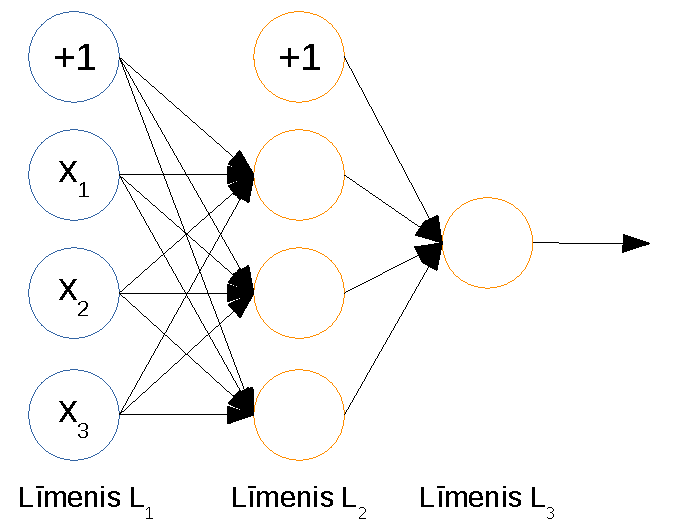
\includegraphics{Img/nn-arhitektura.pdf}
	\caption{Neironu tīkla arhitektūras piemērs.}
	\label{fig:nn}
\end{figure}

Viena no iespējamajām neironu tīklu arhitektūrām ir apskatāma attēlā
\ref{fig:nn} Šeit līmeni $L_1$ sastāda ieejas neironi, kas apzīmē tīklam padotās
ieejas parametru vērtības. Līmeni $L_3$ sastāda neironi (vispārīgā gadījumā tie
var būt vairāki), kuru izejas vērtības tiek atgrieztas kā rezultāts. Pārējos
līmeņus, šoreiz tāds ir tikai viens -- $L_2$ --, sauc par slēptajiem līmeņiem.
Ar $+1$ tiek apzīmēti neironi, kas nesaņem ieejā citu neironu vērtības; tie
atgriež konstanti $1$, un ļauj neironu vērtību un svaru lineārajā kombinācijā
pieskaitīt koeficientu, kas nav atkarīgs no ieejas vērtībām. Bultiņas apzīmē,
kuru neironu atgrieztās vērtības tiek izmantotas kāda neirona ieejā.

Ir pierādīts, ka neironu tīkli darbojas kā universāli funkciju aproksimētāji
\autocite{hornik1991approximation}. Šo apgalvojumu formulē kā universālās
aproksimācijas teorēmu (\textit{universal approximation theorem}). Tā apgalvo,
ka \textit{feed-forward} tipa neironu tīkls (tāds, kas atbilst \ref{fig:nn}
attēla aprakstam) ar vienu slēpto slāni, ar galīgu skaitu neironu un nelineāru
aktivācijas funkciju ir spējīgs aproksimēt nepārtrauktas funkcijas vērtībām, kas
pieder kādai kompaktai $\mathbb{R}^n, n \in \mathbb{N}$ apakškopai. Tas nozīmē,
ka tīkls ar pietiekamu neironu skaitu ir izmantojams patvaļīgu funkciju
aproksimēšanai. Šī ir nozīmīga priekšrocība, salīdzinot ar, piemēram,
lineārajiem funkciju aproksimājiem, un ir pamatā intuīcijai par neironu tīklu
spēju uztvert sakarības MDP optimālajā kontroles stratēģijā. Kā arī spēja
aproksimēt nepārtrauktas funkcijas ir nepieciešama lai funkciju aproksimētājs
būtu spējīgs darboties nepārtrauktās darbību telpās. Turklāt, kā ieejas
parametrus iespējams izmantot MDP stāvokļu mainīgos, izvairoties no atsevišķas
parametru funkcijas ieviešanas, kas ļautu MDP risināšanā izmantot arī tādas
pieejas, kas procesa stāvokli tiešā veidā tulko par veicamo darbību.

Tomēr universālās aproksimācijas teorēma nerisina jautājumu par attiecīgo
parametru algoritmisku iegūšanu, bet tikai par to eksistenci. Praksē uzdevums
vispārīgā gadījumā ir sarežģīts. Neironu tīkla parametru iegūšanu apgrūtina
nepieciešamība izvairīties no lokālajiem minimumiem trenēšanas procesā, tīkla
arhitektūras izvēle, lai izvairītos no pārlieku pielāgošanās treniņa datiem
(\textit{overfitting}) un grūtības, kas saistītas ar labu hiperparametru izvēli
trenēšanas procesam. Turklāt nelineārajiem funkciju aproksimētājiem kopumā ir
mazāk garantiju, ka trenēšanas algoritmus konverģēs uz optimālo risinājumu.
Tomēr pastāv veidi, kā ar šīm problēmām cīnīties -- \textit{overfitting}
problēmu risina ar regularizācijas palīdzību \autocite{sarle1995stopped}
\autocite{srivastava2014dropout}, atsevišķām neironu tīklu arhitektūrām var
veidot mērķa funkciju, kas ir ieliekta, un pastāv metodes optimālo
hiperparametru meklēšanai \autocite{bergstra2011algorithms}. Kopumā neironu
tīklu trenēšanu ir ļoti atvieglojusi \textit{backpropagation} algoritma
ieviešana \autocite{Werbos74} \autocite{Rumelhart1988}. Skatoties uz nelineāriem
funkciju aproksimētājiem kopumā -- atsevišķos gadījumos var arī tikt dotas
konverģences garantijas vismaz lokālā optimuma sasniegšanai
\autocite{bhatnagar2009convergent}.

\iffalse
\section{Parametru pielāgošana}
\subsection{Uz gradientiem bāzētās metodes}
\subsection{Evolucionārās metodes}
\fi

\chapter{Stimulētā mācīšanās} \label{chap:stim}
Stimulētās mācīšanās (SM, angliski -- \textit{reinforcement learning}) pārziņā
ir situācijas, kurās uzdevums jārisina mijiedarbojoties ar apkārtējo vidi. Tā
vietā, lai problēmu risinātu, dodot algoritmam sagatavotus ieejas datus ar
norādītām labākajām darbībām, algoritms mācās no savas pieredzes, izmēģinot
darbības un novērojot saņemto atalgojumu. Vispārīgā gadījumā algoritmam ir
patstāvīgi jāapgūst darbošanās sarežģītos problēmapgabalos, kur darbības labumu
var izvērtēt tikai ilgtermiņā uz priekšu. Citējot \citet{Barto}: "Šie divi
atribūti -- mācīšanās no pieredzes un novēlotais atalgojums -- ir stimulētās
mācīšanās vissvarīgākās raksturiezīmes. Stimulēto mācīšanos definē nevis
mācīšanās metodes, bet gan risināmā problēma." Šīs pieejas ir interesantas, jo
ir tuvas idealizētam skatījumam uz to, kā mācās dzīvnieki vai cilvēks.

De facto modelis stimulētās mācīšanās problēmu formalizēšanai ir \ref{chap:mdp}
nodaļā apskatītie Markova izvēles procesi. Tiek pieņemts, ka aģentam sākotnēji
nav pieejama nekāda informācija par procesu, izņemot, kādām kopām pieder procesa
stāvokļi un pieejamās darbības.

Dažādās konceptuālās MDP risināšanas pieejas, kas izriet no Bellmana
vienādojumiem ir apskatītas nodaļā \ref{chap:mdp} Šajā nodaļā tiks pievērsta
padziļināta uzmanība stratēģijas aproksimēšanas algoritmiem. Bet vispirms
jāsniedz īss ieskats \textit{temporal difference} soļu izmantošanu algoritmos.

\section{Temporal difference soļi} \label{chap:td}
\textit{Temporal difference} (TD) soļi tiek izmantoti stāvokļu vērtības
funkcijas aproksimācijā. Šis paņēmiens ir idejiski tuvāks vērtības
aproksimācijas metodēm, bet, kā vēlāk redzēsim, ir izmantojams arī
\textit{actor-critic} metodēs, lai iegūtu $V^*$ aproksimāciju. Pastāv dažādas
idejas variācijas, kas ir pamatā vairākiem vērtību aproksimācijas algoritmiem,
kas tiek klasificēti zem \textit{TD learning} vārda, bet pamatideja ir
vienkārša. TD soļiem tabulārajā formā stāvokļu vērtību funkcija tiek pielāgota,
izmantojot vienādojumu
\[
	V_{t+1}(s_t) = V_t + \alpha_t(s_t) \delta_t,
\]
kur $\delta_t = r_{t} + \gamma V_t(s_{t + 1}) - V_t(s_t)$ un $\alpha_t(s_t) \in
[0,1]$ ir soļa lieluma parametrs.
Nepārtrauktai stāvokļu vērtību funkcijai TD soļa pielietošana ir saistīta ar
\textit{gradient ascent} soļa veikšanu funkcijas parametriem. Ja ir dota
parametrizēta vērtību funkcija $V:S \times \Theta \rightarrow \mathbb{R}$, tad
TD solis tiek veikts funkcijas parametriem atbilstoši vienādojumam
\[
	\theta_{t+1} = \theta_t + \alpha_t(s_t) \delta_t \nabla_\theta V_t(s_t).
\]
Uzskatāmības labad ieviesīsim jaunu apzīmējumu, kas šo pierakstu vienkāršos.
Ar
\[
	A_{t+1}(x) \xleftarrow{\alpha} B_t
\]
apzīmēsim $A_t$ pielāgošanu, nākamajā laika momentā $A_t(x)$ tuvinot vērtības
$B_t$ virzienā apmērā $\alpha$, kur $\alpha \in [0,1]$. Ja funkcija ir uzdota
tabulārā formā (tā ir diskrēta), tad iepriekšējā izteiksme apzīmē soli
\[
	A_{t+1}(x) = A_t(x) + \alpha(A_t(x) - B_t).
\]
Ja funkcija $A(x)$ ir nepārtraukta, un ir parametrizēta ar kādu papildus vektoru
$\theta$, tad ar pierakstu saprotam
\[
	\theta_{t+1} = \theta_t + \alpha \left(B_t - A_t(x)\right) \nabla_\theta A_t(x),
\]
ko var interpretēt, kā \textit{gradient descent} soļa veikšanu parametriem
$\theta$ pa $B_t$ un $A_t(x)$ starpības kvadrāta funkcijas vērtību. Tas ļauj
pārrakstīt TD soli kā
\[
	V_{t+1}(s_t) \xleftarrow{\alpha_t(s_t)} r_t + \gamma V_t(s_{t + 1}).
\]

Vairāk par TD metodēm var lasīt \autocite{Hasselt2012}.

\section{Stratēģijas aproksimācija}
Kā iepriekš minēts, stratēģijas aproksimācijas pieeju raksturo stratēģijas
funkcijas $\pi$ glabāšana tiešā veidā un pielāgošana algoritma darbības laikā,
lai to tuvinātu optimālajai stratēģijai $\pi^*$. Tas ļauj izvairīties no
grūtībām, ar ko nākas saskarties tīrajās vērtību aproksimācijas metodēs, tā kā
nav nepieciešams papildus darbs, lai atrastu labāko stratēģiju algoritma
darbības beigās, vai arī labāko gājienu kādam stāvoklim algoritma darbības
laikā. Tas ir nozīmīgs ieguvums nepārtrauktās darbību telpās, jo nav jāveic
darbību telpas diskretizācija, un ir pat iespējams lietot procesa stāvokļus
tiešā veidā bez atsevišķa parametru iegūšanas soļa.
%TODO varbūt vajag pieminēt ATARI rakstu un pateikt, ka gribu darīt tāpat, kā
%viņi ar value funkciju.

Šeit mēs lietosim pielāgotu stratēģijas funkcijas definīciju, lai pieļautu
iespēju lietot stratēģiju nosakošu parametru vektoru. Funkcija būs formā $\pi: S
\times A \times \Psi \rightarrow [0,1]$, kur $\pi(s, a, \psi)$ norāda varbūtību
atrodoties stāvoklī $s$ veikt darbību $a$ pie stratēģijas parametru vērtībām
$\psi \in \Psi \subseteq \mathbb{R}^{D_\Psi}$.

%TODO šeit iespējams vajag Actor-only virsrakstu
\subsection{Actor-only metodes}
 
Lai stratēģijas aproksimēšanai varētu izmantot kādu parametrizētu funkciju,
nepieciešams ieviest veidu, kā pielāgot tās parametrus algoritma darbības laikā,
ņemot vērā saņemto atalgojumu. Standarta pieeja ir izmantot \textit{gradient
  ascent} soļus pa $V^\pi$ sagaidāmās vērtības funkciju
\autocite{williams1992simple} \autocite{sutton2000policy}
\autocite{Hasselt2012}. Citiem vārdiem -- stratēģijas parametri tiek pielāgoti
tā, lai pieaugtu funkcijas $V^\pi$, kā tā ieviesta \eqref{eq:vpi}, sagaidāmā
vērtība. Stratēģijas parametru pielāgošanas solis (\textit{batch} gadījumā) ir
\[
	\psi_{k+1} = \psi_k + \beta_k \nabla_\psi E \left\{V^\pi(s_t)\right\} =
  \psi_k + \beta_k \nabla_\psi \int_{s \in S} P(s_t = s) V^\pi(s)\ ds,
\]
kur $P(s_t = s)$ norāda varbūtību, ka aģents laikā $t$ atrodas stāvoklī $s$, un
$\beta_k \in [0,1]$ ir mācīšanās soļa izmērs. Pastāv arī alternatīva, kur tiek
lietots \textit{gradient ascent} stohastiskais variants, kas ļauj parametru
vērtības pielāgot katrā solī
\begin{equation} \label{eq:stohgrad}
	\psi_{t+1} = \psi_t + \beta_t(s_t) \nabla_\psi V^\pi(s_t).
\end{equation}

Šeit \textit{actor-only} algoritmi sastopas ar problēmu. Veicot \textit{gradient
  ascent} soļus pa $V^\pi$ funkciju (vai sagaidāmās vērtības funkciju)
diferencējamā funkcija \textit{actor-only} piegājienā nav pieejama. Ar to
iespējams tikt galā, ar vairākām matemātiskām manipulācijām, kas šeit izlaistas,
izsakot $\nabla_\psi V^\pi(s_t)$ ar $\pi$ funkciju
\begin{equation} \label{eq:nablav}
	\nabla_\psi V^\pi(s_t) = E \left\{R_k(s_t)
    \left(\sum\limits_{j=t}^{T_k - 1} \nabla_\psi \log \pi(s_j, a_j, \psi) \right)
  \right\}
\end{equation}

Sagaidāmā vērtība šajā un atvasinātajās metodēs tiek iegūta ar \textit{Monte
  Carlo} metodēm \autocite{halton1970retrospective}. Īsumā -- meklējamā vērtība
tiek novērtēta ar vairāku nejaušu paraugu palīdzību. \textit{Monte Carlo}
metodes pielietojot gradienta aprēķiniem \textit{actor-only} piegājienā, ir
novērots, ka tās saistās ir lielas dispersijas ieviešanu rezultātos. Tas var
būtiski negatīvi ietekmēt laiku, kas algoritmam ir nepieciešams, lai sasniegtu
rezultātu. Ar dažādiem paņēmieniem ar šo efektu ir iespējams cīnīties, bet, kā
vēlāk redzēsim, \textit{actor-critic} piegājienā no šo metožu izmantošanas ir
iespējams izvairīties vispār. %TODO: kas atrisina ar to saistītās problēmas.?

\textit{Actor-only} metodēm mēs tālāk šeit nesekosim.
Vispārīgs pārskats ir dots \autocite{Hasselt2012}.
 
\subsection{Actor-critic metodes}
\textit{Actor-critic} metodes ar iepriekšējā sadaļā norādītajiem ierobežojumiem
cīnās līdztekus ar $\pi^*$ aproksimējot arī $V^*$. Gadījumā, kad parametru
vektora $\psi$ pielāgošanai tiek izmantoti \textit{gradient ascent} soļi pa
$V^\pi$, tas ļauj iztikt bez vienādojumā \eqref{eq:nablav} redzamā lieluma
novērtēšanas ar \textit{Monte Carlo} metodēm, jo var parādīt, ka tā vietā var
novērtēt $Q^\pi(s_t, a_t) - V^\pi(s_t)$ ar lielumu $\delta_t = r_{t} + \gamma
V_t(s_{t+1}) - V_t(s_t)$. Lielums $\delta_t$ tiek dēvēts par \textit{temporal
  difference} (TD) \textit{error}. Tas ļauj stratēģijas gradientu novērtēt ar
$\delta_t \nabla_\psi \log \pi(s_t,a_t,\psi_t)$ \autocite{sutton2000policy},
aizstājot \eqref{eq:stohgrad} ar
\begin{equation} \label{eq:psi}
	\psi_{t+1} = \psi_t + \beta_t(s_t) \delta_t \nabla_\psi \log \pi(s_t,a_t,\psi_t)
\end{equation}
kā stratēģijas parametru pielāgošanas soli.

Līdz šim ir apskatītas pieejas stratēģijas parametrus pielāgo, cenšoties
paaugstināt $V^\pi$ sagaidāmo vērtību. Alternatīva ir parametrus pielāgot,
cenšoties samazināt stratēģijas $\pi$ atšķirības no optimālās stratēģijas
$\pi^*$. Citiem vārdiem -- ņemt vērā pašreizējās stratēģijas optimālo gājienu
prognožu kļūdas. Šī ideja ir būtiska \textit{continuous action-critic learning
  automaton} (CACLA) algoritmam, un nošķir to no vairuma citu
\textit{actor-critic} metožu.

\chapter{CACLA algoritms}
CACLA algoritma pamatā ir vienkārša ideja -- ja veiktā darbība paaugstina
stāvokļa vērtības novērtējumu, tad šim stāvoklim ir derīgi pielāgot stratēģiju
veiktās darbības virzienā, jo tā potenciāli var novest pie lielāka kopējā
atalgojuma.
%Paralēli tam, algoritms katrā solī uzlabo savu stāvokļu vērtības novērtējumu.
%Laika gaitā stāvokļu vērtības novērtējums konverģē uz  Rezultātā algoritma
%stratēģija ar vien vairāk tuvojas optimālajai.
Algoritms glabā funkciju $V:S \times \Theta \rightarrow \mathbb{R}$ -- kritiķi
-- un $Ac : S \times \Psi \rightarrow A$ -- aktieri. Sasaistot apzīmējumus ar
ierastajiem -- $V$ tagad tiek \textit{parametrizēta} ar kādu vektoru $\theta \in
\Theta$, kas ļaus pielāgot funkcijas vērtības algoritma darbības laikā.
Apzīmēsim $V_t(s_t) = V(s_t, \theta_t)$ un $Ac_t(s_t) = Ac(s_t, \psi_t)$.
Aktieris katrā solī dotajam stāvoklim $s_t$ sniedz darbību $Ac(s_t, \psi_t)$.
Lai nodrošinātu darbību telpas izpēti, nepieciešams, lai galā izmantotā darbība
atšķiras no ieteiktās, jeb $a_t \neq Ac(s_t, \psi_t)$. To var darīt, piemēram,
ņemot $\pi(s_t, \psi_t)$ kā \textit{normālsadalījumu} ar centru $Ac(s_t,
\psi_t)$. Kad ir iegūta veicamā darbība $a_t$, novēro atalgojumu $r_t$ un veic
standarta TD soli vērtību funkcijai, kā tas aprakstīts sadaļā \ref{chap:td}
\[
	V_{t+1}(s_t) \xleftarrow{\alpha_t(s_t)} r_t + \gamma V_t(s_{t + 1}).
\]
Ja $a_t$ veikšana ir palielinājusi $s_t$ vērtības novērtējumu, t.i., ja
$V_{t+1}(s_t) > V_t(s_t)$, tad pielāgo aktieri darbības $a_t$ virzienā
\[
	Ac_{t+1}(s_t) \xleftarrow{\beta_t(s_t)} a_t.
\]


\begin{spacing}{1}
\begin{algorithm}
\caption{CACLA pseidokods}\label{alg:cacla}
inicializē $\theta_0, \psi_0, s_0$ \\
\For{$t \in \{0,1,2,\ldots\}$}{
	ņem $a_t$ ar izkliedi ap $Ac_t(s_t)$ \\
	veic $a_t$, novēro $r_t, s_{t+1}$ \\
	\eIf{$s_{t+1}$ ir gala stāvoklis}{
		$V_{t+1}(s_t) \xleftarrow{\alpha_t(s_t)} r_t$ \\
		ņem jaunu $s_{t+1}$ ($s_{t+1}$ ir sākumstāvoklis nākamajā trenēšanas epizodē)
	}{
		$V_{t+1}(s_t) \xleftarrow{\alpha_t(s_t)} r_t + \gamma V_t(s_{t + 1})$
	}
	\If{$V_{t+1}(s_t) > V_t(s_t)$}{
		$Ac_{t+1}(s_t) \xleftarrow{\beta_t(s_t)} a_t$
	}
}
\end{algorithm}
\end{spacing}

\FloatBarrier

CACLA pseidokods ir dots algoritmā \ref{alg:cacla} Pārfrāzēsim to saistībā ar
konkrētiem stratēģijas un stāvokļu vērtību funkcijas aproksimētājiem --
izmantosim divus neironu tīklus, ko sauksim attiecīgi par $NTA_{\psi_t}$ un
$NTV_{\theta_t}$, apakšdrukā norādot izmantojamos parametrus. Algoritms sāk,
inicializējot (piemēram, ģenerējot nejaušas vērtības, kas tuvas $0$) $NTV$
parametrus $\theta_0$ un $NTA$ parametrus $\psi_0$, kā arī izvēlas sākuma
stāvokli $s_0$, kas var būt skalāru vērtību vektors. Tiek sākta neironu tīklu
trenēšana, un katrā laika momentā $t$ tiek paveikts:
\begin{itemize}
	\item darbina $NTA{\psi_t}(s_t)$, iegūstot stāvoklim $s_t$ labāko zināmo
    darbību (kas var būt skalāru vērtību vektors); lai nodrošinātu darbību
    telpas izpēti, veicamā darbība  $a_t$ tiek ņemta ar izkliedi ap
    $NTA_{\psi_t}$ atgriezto vektoru;
	\item veic darbību $a_t$, un novēro stāvokli $s_{t+1}$, uz kuru sistēma
    pāriet, un saņemto atalgojumu $r_t$;
	\item ja $s_{t+1}$ ir gala stāvoklis:
	\begin{itemize}
		\item[--] veic stohastiskā \textit{gradient descent} soli $NTV$ parametriem
      $\theta_t$ pa funkciju, kas izsaka $\left(NTV_{\theta_t}(s_t) -
        r_t\right)^2$ atkarībā no $\theta_t$; iegūst $\theta_{t+1}$;
        %TODO šis jādziens jāpaskaidro 2. nodaļā
		\item[--] izvēlas nākamās epizodes sākumstāvokli $s_{t+1}$;
	\end{itemize}
	\item citādi:
	\begin{itemize}
		\item[--] veic stohastiskā \textit{gradient descent} soli $NTV$ parametriem
      $\theta_t$ pa funkciju, kas izsaka ${\left(NTV_{\theta_t}(s_t) - \left(r_t
          + \gamma NTV_{\theta_t}(s_{t+1}) \right) \right)}^2$ atkarībā no
      $\theta_t$; iegūst $\theta_{t+1}$;
	\end{itemize}
	\item ja $NTV_{\theta_{t+1}}(s_t) > NTV_{\psi_t}(s_t)$ ($s_t$ vērtība
    palielinājusies):
	\begin{itemize}
		\item[--] veic stohastiskā gradient \textit{descent} soli $NTA$ parametriem
      $\psi_t$ pa funkciju, kas izsaka ${\left(NTA_{\psi_t}(s_t) - a_t\right)}^2$
      atkarībā no $\psi_t$; iegūst $\psi_{t+1}$;
	\end{itemize}
	\item atkārto.
\end{itemize}

CACLA algoritms ir ieviests \autocite{Hasselt2007}. Tas radies, pielāgojot
\textit{actor-critic learning automaton} (ACLA) algoritmu nepārtrauktām darbību
telpām. To darbībā ir vairākas līdzības, piemēram $Ac_t$ pielāgošana, ņemot vērā
tikai TD izmaiņas zīmi, nevis konkrēto vērtību, kā tas tiek darīts vairumā citu
\textit{actor-critic} algoritmu. Šai pieejai ir vairākas priekšrocības
\autocite{Hasselt2007}. Tā dara algoritmu noturīgu pret troksni novērojumos
trenēšanas laikā. CACLA algoritma gadījumā tā padara stāvokļu vērtību funkciju
invariantu pret dažāda veida mērogošanu. Kā papildus ieguvums ir tas, ka
algoritmu ir viegli implementēt. Kā arī šis ir viens no iemesliem, kāpēc
algoritmu ir viegli izmantot nepārtrauktām darbību telpām un savietot ar,
piemēram, neironu tīkliem.

Zīmīgi ir arī tas, ka TD izmaiņas apjoma ignorēšana var dot mācīšanās ātruma
pieaugumu. Tas ir novērojams, kad stāvokļu vērtības funkcijas parametri nonāk
apgabalos ar mazām izmaiņām funkcijas vērtību telpā. Šādos apgabalos TD izmaiņas
apjoms ir mazs, un klasiskajā gadījumā tas noved pie mazas izmaiņas aktiera
parametros. Intuīcija saka, ka pielāgojot aktiera uzvedību, attālums līdz jaunai
daudzsološai darbībai ir nozīmīgāks nekā stāvokļa vērtības pieaugums, ko jaunā
uzvedība sniegtu sniegtu.

Šiem apsvērumiem par labu runā arī novērojumi \autocite{Hasselt2007}. Rakstā
CACLA algoritms tiek salīdzināts ar citiem nepārtrauktu darbības telpu
\textit{actor-critic} algoritmiem. Novērojumi rāda, ka CACLA daudz ātrāk
sasniedz labas stratēģijas. Apskatīts tiek arī CACLA variants, kas veic papildus
aktiera pielāgošanas soļus, ja TD izmaiņa ir bijusi liela attiecībā pret
standartnovirzi, kas noved pie vēl ātrākas labas stratēģijas sasniegšanas.

Tā kā TD izmaiņas apmērs nav būtisks, aktiera parametrus var pielāgot, ņemot
vērā tikai kļūdu darbību telpā. Izmantotais pielāgošanas solis $Ac_{t+1}(s_t)
\xleftarrow{\beta_t(s_t)} a_t$ ir ekvivalents \textit{gradient descent} soļa
veikšanai parametriem $\theta$ pa $B_t$ un $A_t(x)$ starpības kvadrāta funkcijas
vērtību. Citiem vārdiem -- aproksimācijai lietojot neironu tīklus, to parametru
pielāgošanai pie pozitīvas TD izmaiņas var lietot standarta stohastiskā
{gradient descent} pielāgošanas soli. Tas atbilst no mašīnmācīšanās aizgūtajai
intuīcijai par neironu tīklu parametru pielāgošanu.

Atšķirībā no ACLA algoritma, CACLA nepielāgo aktieri, ja TD izmaiņa ir bijusi
negatīva. Tādējādi tiktu veiktas izmaiņas virzienā prom no izmēģinātās darbības,
t.i., kādas citas neizmēģinātas darbības virzienā. Šādu pieeju pamato, apskatot
gadījumu, kad algoritms, pieņemsim, jau ir sasniedzis optimālo stratēģiju un
stāvokļu vērtības funkciju. Šajā gadījumā neviena darbība nenoved pie pozitīva
TD izmaiņas un algoritms virzās prom no optimālās stratēģijas. Tas ir arī
empīriski pārbaudīts \autocite{Hasselt2007}. CACLA modifikācijai, kas veic
izmaiņas stratēģijā arī, kad TD izmaiņa ir bijusi negatīva, ir novērojama
pasliktināšanās algoritma darbībā.

Citā darbā CACLA algoritms tiek salīdzināts arī ar vērtību aproksimācijas
algoritmiem diskrētās darbību telpās \autocite{Hasselt2009}. Tiek parādīts, ka
pārbaudītajos domēnos CACLA ir izteiktas priekšrocības attiecībā pret diskrētu
darbības telpu algoritmiem, kā \textit{Q-learning} un \textit{Sarsa},
neskatoties uz to, ka CACLA darbības tiek noapaļotas uz tuvākajām pieļaujamajām.
Interesants novērojums minētajā darbā ir, ka CACLA parāda spējas vispārināt
apgūto stratēģiju līdzīgiem uzdevumiem. Tika novērots, ka darbību telpas
samazināšana \textit{cart-pole} uzdevumā, atstājot tikai 2 pieejamās darbības,
neprasīja algoritma pārtrenēšanu, atšķirībā no pārējiem algoritmiem. Tas tiek
skaidrots ar priekšrocībām, ko sniedz nepārtrauktas darbību telpas izmantošana.
Diskrēto algoritmu rezultātu kritums ir skaidrojams ar to, izmestās darbības
tika apgūtas, ka atsevišķas sastāvdaļas stratēģijā. Tā kā algoritms ir
iemācījies uz tām paļauties lielā daļā gadījumu, tad to izmešana būtiski
negatīvi ietekmē sniegumu. CACLA neiemācās paļauties uz konkrētām darbībām --
stratēģija ir vispārīga, jo ir ietvertas sakarības darbību telpā. Tomēr
interesanti, ka ieguvums ir arī attiecībā pret pārējiem testētajiem nepārtraukto
darbības telpu algoritmiem.

%\subsubsection{CACLA darbības analīze literatūrā}
\chapter{CCACLA algoritms}\label{chap:ccacla}
CACLA algoritms izmanto divus neironu tīklus, no kuriem viens aproksimē optimālo
stratēģiju, bet otrs -- stāvokļu vērtības funkciju. Abu neironu tīklu parametri
tiek pielāgoti, tiem savstarpēji mijiedarbojoties algoritma darbības laikā --
stāvokļu vērtības funkcija ir atkarīga no optimālās stratēģijas aproksimācijas,
jo tā nosaka, kādas darbības tiek veiktas katrā stāvoklī, kas laika gaitā
ietekmē stāvokļu vērtību, savukārt optimālās stratēģijas aproksimācija tiek
pielāgota atkarībā no stāvokļu funkcijas izmaiņām, ņemot vērā, vai stratēģijas
noteiktā darbība dotā stāvoklī pēc izpildes palielina stāvokļa vērtību. Šīs
savstarpējās mijiedarbības rezultātā algritms ir spējīgs mācīties, bet rodas
jautājums, vai šādi netiek darīts lieks darbs. Gan stāvokļu vērtības funkcijas
aproksimācijas $V$ gan optimālās stratēģijas funkcijas aproksimācijas $A$ domēns
ir vides stāvokļu telpa $S$. Ir saprātīgi pieņemt, ka abu funkciju vērtības
varētu noteikt līdzīgas pazīmes stāvokļu telpā. Abu attiecīgo neironu tīklu
otrais slānis varētu būt trenēšānas rezultātā iemācījies izejā dot līdzīgus
aktivācijas vienos un tajos pašos stāvokļus, tāpēc rodas jautājums, vai abus
tīklus nav iespējams apvienot.

Skatījumu uz neironu tīkliem kā hierarhiskiem pazīmju izgūšanas rīkiem sniedz
pēdējā laikā lielu popularitāti ieguvusī dziļās mācīšanās paradigma. Tās pamatā
ir ideja, ka daudzos dažādos ar reālo pasauli saistītos domēnos, piemēram, attēlu
vai runas atpazīšānā, dabīgās valodas apstrādē u.c., pētāmos objektus ir
iespējams raksturot ar hierarhisku vairāklīmeņu pazīmju kopumu \autocite{Lecun2015}. Tas ļauj
izmantot vairākļīmeņu neironu tīklus šo pazīmju izgūšanai. %TODO piemērs
Lai arī šajā darbā apskatītajās stimulētās mačīšanās problēmas atāvokļu telpas
nav tik sarežģītas, lai būtu nepieciešamība izmanot dziļus neironu tīklus, tomēr
arī uz sekliem neironu tīkliem var raudzīties kā uz ierīcēm, kas izgūst zema
līmeņa pazīmes, ko pēdējais tīkla līmenis ir iemācījies apstrādāt. Šis skatījums
rada papildus motivāciju pētīt, vai nav iespējams lietderīgi izmantot CACLA
algoritmā izmantoto neironu tīklu apakšējo līmeņu izgūto pazīmju īpatnības.

Šajā nodaļā tiks apskatītas vairākas CACLA algoritma modifikācijas, kuras to
kopīgo īpašību dēļ autors ievieto vienā algoritmu grupā ar kopīgo nosaukumu
Combined CACLA, jeb CCACLA. Visu algoritmu kopīgā iezīme, kas tos atšķir no
iepriekš apskatītā CACLA algoritma ir viena neironu tīkla izmantošana gan
vērtību funkcijas $V$ gan optimālās stratēģijas funkcijas $A$ aproksimācijai.
Tiek apskatīti vairāki šī algoritma paveidi, kas ietver modifikācijas tajā, kāda
informācija tiek izmantota tīkla trenēšanai.

%TODO jāpasaka kaut kas par to, ka tiek šeit CACLA un CCACLA algoritmi tiek
%aprakstīti tikai kontekstā ar neironu tīkliem. Idejas par kopīgu slāņu
%izmantošanu gan aktiera gan kritiķa komponentei dabīgāk sasaistāmas ar neironu
%tīkliem kā šo komponenšu implementācijām. Pastāv tomēr arī iespējas
%alternatīvam formulējumam, kas izmanto patvaļīgus funkciju aproksimatorus. Šajā
%interpretācijā uzdevums pārvēršas par mēģinājumu atrast kādu parametru
%komplektu, ko šie funkciju aproksimētāji varētu dalīt savā starpā.
\section{CCACLA pamatalgoritms}
CCACLA vienkāršākais variants, kas vismazāk atšķiras no par pamatu ņemtā CACLA
algoritma, izmanto funkciju 
\begin{equation}
  Av_\Theta:S \rightarrow A \times \mathbb{R},
\end{equation}
lai stāvoklī $s$ paredzētu gan optimālo darbību $a$, gan stāvokļa vērtību $v$ kā
$Av_\Theta(s) = (a, v)$. Funkcija $Av_\Theta$ tiek realizēta ar
neironu tīklu, kas sastāv no ieejas slāņa, slēptā slāņa, un diviem izejas
slāņiem, kas slēptā slāņa aktivācijas pārvērš, respektīvi, optimālajā darbībā
$a$ un stāvokļa vērtībā. Šīs vērtības tad attiecīgi var izteikt, kā
\begin{equation}\label{eq:ccacla-act}
  v = V(s), V(s) = f_a\left(f_h(s^T \cdot W_h) \cdot W_a\right)
\end{equation} un
\begin{equation}\label{eq:ccacla-val}
  a = Ac(s), Ac(s) = f_v\left(f_h(s^T \cdot W_h) \cdot W_v\right)
\end{equation}, kur $s$ ir
ieejas vektors (stāvoklis), $W_h$ ir slēptā slāņa svaru matrica, $W_a$ ir
darbības slāņā svaru matrica, $W_v$ ir vērtības slāņa svaru matrica, $f_h$ ir
slēptā slāņā aktivācijas funkcija, $f_a$ ir darbības slāņā aktivācijas funkcija
un $f_v$ ir vērtības slāņā aktivācijas funkcija. Ar ieviestajiem mainīgajiem
varam arī izteikt funkciju $Av$
\begin{equation}\label{eq:ccacla-actval}
  Av(s) = \left(f_a(h^{(1 \ldots D(A))}), f_v(h^{(D(A) + 1)})\right), \text{ kur } 
  h = f_h\left(f_h(s^T \cdot W_h) \cdot W_v\right)
\end{equation}
%TODO: pateikt, ka bias vērtības ir iekļautas W

Citos aspektos CCACLA pamatalgoritms neatšķiras no CACLA. Šādi izteiktas funkcijas
$V(s)$ un $Ac(s)$ ļauj izmantot jau iepriekš definēto CACLA algoritmu <reference
uz cacla pseidokodu>. Atbilstoši vienādojumam \ref{eq:ccacla-actval} iespējams
arī definēt optimizētu versiju, kas izmanto faktu, ka $a$ un $v$ iespējams
izrēķināt vienlaicīgi. Tas parādīts algoritmā \ref{alg:ccacla-basic}.

\begin{spacing}{1}
\begin{algorithm}
\caption{CACLA pseidokods}\label{alg:ccacla-basic}
inicializē $\theta_0, \psi_0, s_0$ \\
$(a_0', v_0) := Av_0(s_0)$ \\
ņem $a_0$ ar izkliedi ap $a_0'$ \\
\For{$t \in \{1,2,\ldots\}$}{
	veic $a_{t-1}$, novēro $r_{t-1}, s_t$ \\
  $(a_t', v_t) := Av_t(s_t)$ \\
	ņem $a_t$ ar izkliedi ap $a_t'$ \\
	\eIf{$s_t$ ir gala stāvoklis}{
		$V_t(s_{t-1}) \xleftarrow{\alpha_{t-1}(s_{t-1})} r_{t-1}$ \\
		ņem jaunu $s_t$ ($s_t$ ir sākumstāvoklis nākamajā trenēšanas epizodē)
    % TODO: šeit jāiestata arī a un v (vai arī jāpievieno ārējais cikls, un šeit
    % var rakstīt goto 1)
	}{
		$V_t(s_{t-1}) \xleftarrow{\alpha_t(s_{t-1})} r_{t-1} + \gamma v_t$
	}
	\If{$r_{t-1} + \gamma v_t > v_{t-1}$}{
		$V_t(s_{t-1}) \xleftarrow{\beta_t(s_{t-1})} a_{t-1}$
	}
}
\end{algorithm}
\end{spacing}

% Algoritma \ref{alg:ccacla-basic} 9. un 14. rindiņā nepieciešams veikt gradient
% descent soļus funkcijām \ref{eq:ccacla-act} un \ref{eq:ccacla-val}, kam
% nepieciešami šo funkciju diferenciāļi.
% \begin{equation}
%   \frac{\partial V}{\partial s} = 
% \end{equation}
%TODO varbūt jāpastāsta par bakcprop. skat: https://en.wikipedia.org/wiki/Backpropagation

\section{CCACLA ar stāvokļa paredzēšanu}
Kā tika minēts iepriekš, interesi rada jautājums, vai ir iespējams ar kādas
papildinformācijas palīdzību trenēšanas laikā likt stimulētās mācīšanās aģentam
veidot iekšēju vides modeli ar mērķi paātrināt mācīšanos. Šajā nolūkā tiek
ieviests CCACLA algoritms ar stāvokļa paredzēšanu, kas no iepriekš aprakstītā
CCACLA pamatalgoritma atšķiras ar to, ka kombinētajam neironu tīklam tagad ir
jāparedz arī nākamais stāvoklis, kurā nonāks aģents pēc paredzētās optimālās
darbības veikšanas. Tas noved pie funkcijas $Aov$ 
\begin{equation}
  Aov_\Theta:S \rightarrow A \times S \times \mathbb{R}
\end{equation}
Līdz ar funkciju \ref{eq:ccacla-act} un \ref{eq:ccacla-val} tagad ieviesīsim arī
funkciju $St$, kas vēlāk tiks izmantota, CCACLA' algiritma pseidokodā, lai
atvieglotu gradient descent soļu pierakstu
\begin{equation}\label{eq:ccacla-obs}
  s' = St(s), St(s) = f_s(f_h(s^T \cdot W_h) \cdot W_a)
\end{equation} 
, kur $W_S$ ir nākamā stāvokļa paredzēšanas slāņa svaru matrica, un $f_S$ ir
slāņa aktivācijas funkcija.
Analogi vienādojumam \ref{eq:ccacla-actval} tagad varam definēt funkciju $Aov$,
kas parāda, kā funkciju \ref{eq:ccacla-act}, \ref{eq:ccacla-act} un
\ref{eq:ccacla-act} apvieno vienā neironu tīklā.
\begin{multline}\label{eq:ccacla-actobsval}
  Aov(s) = \left(f_a(h^{(1 \ldots D(A))}),
                 f_s(h^{(D(A) + 1 \ldots D(A) + D(S))}),
                 f_v(h^{(D(A) + D(S) + 1)})\right), \\
  \text{ kur } h = f_h\left(f_h(s^T \cdot W_h) \cdot W_v\right)
\end{multline}

Lai aprakstītu CACLA' pseidokodā pietrūkst vēl viena funkcija. Atšķirība no
CCACLA pamatalgoritma ir tajā, ka tagad nākas šķirot gadījumus, kuros
trenēšanai kā ieejas dati ir pieejama stāvokļa vārtība, kuros -- nākamais
stāvoklis, kuros -- optimālā darbība, un kuros ir pieejama kāda kombinācija no
minētajām vērtībām. Tādēļ nākas ieviest funkciju, nākamā stāvokļa paredzēšānai
un esošā stāvokļa vērtības paredzēšanai.
\begin{multline}\label{eq:ccacla-obsval}
  Ov: S \rightarrow S \times \mathbb{R},
        Ov(s) = \left(f_s(h^{(D(A) + 1 \ldots D(A) + D(S))}),
                 f_v(h^{(D(A) + D(S) + 1)})\right), \\
  \text{ kur } h = f_h\left(f_h(s^T \cdot W_h) \cdot W_v\right)
\end{multline}
Ar tās un iepriekš definēto funkciju paldīzību varam ideju definēt precīzāk
algoritmā \ref{alg:ccacla-state}.

\begin{spacing}{1}
\begin{algorithm}
\caption{CACLA pseidokods}\label{alg:ccacla-state}
inicializē $\theta_0, \psi_0, s_0$ \\
$(a_0', v_0) := Av_0(s_0)$ \\
ņem $a_0$ ar izkliedi ap $a_0'$ \\
\For{$t \in \{1,2,\ldots\}$}{
	veic $a_{t-1}$, novēro $r_{t-1}, s_t$ \\
  $(a_t', v_t) := Av_t(s_t)$ \\
	ņem $a_t$ ar izkliedi ap $a_t'$ \\
	\eIf{$s_t$ ir gala stāvoklis}{
    \eIf{$r_{t-1} + \gamma v_t > v_{t-1}$}{
      $Av_t(s_{t-1}) \xleftarrow{\alpha_{t-1}(s_{t-1})} (a_{t-1}, r_{t-1})$ \\
    }{
      $V_t(s_{t-1}) \xleftarrow{\alpha_{t-1}(s_{t-1})} r_{t-1}$ \\
    }
		ņem jaunu $s_t$ ($s_t$ ir sākumstāvoklis nākamajā trenēšan as epizodē)
    % TODO: šeit jāiestata arī a un v (vai arī jāpievieno ārējais cikls, un šeit
    % var rakstīt goto 1)
	}{
    \eIf{$r_{t-1} + \gamma v_t > v_{t-1}$}{
      $Aov_t(s_{t-1}) \xleftarrow{\alpha_t(s_{t-1})} (a_{t-1}, s_t, r_{t-1} + \gamma v_t)$
    }{
      $Ov_t(s_{t-1}) \xleftarrow{\alpha_t(s_{t-1})} (s_t, r_{t-1} + \gamma v_t)$
    }
	}
}
\end{algorithm}
\end{spacing}

\section{CCACLA ar paredzēšanu nākotnē}
Iepriekšējā sadaļā aprakstītais CCACLA algoritms ar stāvokļa paredzēšānu ir
veidots ar mērķi trenēšanas laikā likt stimulētās mācīšanās aģentam veidot
iekšēju vides modeli. Algoritma formulējumā gan var ievērot kādu īpatnību.
Funkcija $Aov(s) = (a, s', v)$ dotam stāvoklim $s$ atgriež optimālo darbību $a$
un stāvokli $s'$, kurā vide (visticamāk) nonāks pēc $a$ veikšanas, tomēr
atgrieztā vērtība $v$ atbilst stāvoklim $s$, nevis $s'$. Vērtības $v$
sasaistīšana ar $s$ atbilst oriģinālajam CACLA algoritma formulējumam, tomēr
varētu uzdot jautājumu, vai, liekot algoritma neironu tīklam paredzēt gan nākamo
stāvokli gan šī stāvokļa vērtību, nevar uzlabot algoritma darbību. Sasaistot šo
ideju ar iepriekš izteikto mērķi mēģināt rast veidus, kā stimulētās mācīšanās
aģentam likt veidot iekšēju vides modeli, ideju var intuitīvi pamatot, sakot, ka
nākamā stāvokļa vērtības paredzēšanai šāds modelis ir nepieciešams.

Ņemot vērā iepriekšējos apsvērumus, veidosim algoritma CCACLA variantu ar
paredzēšanu nākotnē. Šis algoritma variants izmantos tādu pat neirona tīkla
struktūru, kā CCACLA ar stāvokļa paredzēšanu. Atšķirības būs tikai tīkla
trenēšanas procesā, kā rezultātā tiks pielāgoti funkciju $V$, $Ov$ un $Aov$
parametri tā, lai stāvokļa vērtība, ko atgriež šīs funkcijas, atbilstu stāvoklim
$s'$ nevis $s$. Viennozīmības labad CCACLA algoritmā ar paredzēšanu nākotnē
apzīmēsim šīs funkcijas, attiecīgi kā $V'$, $Ov'$ un $Aov'$. Šīs funkcijas
nemainīgi tiek definētas atbilstoši
vienādojumiem~\eqref{eq:ccacla-val}~\eqref{eq:ccacla-obsval}~\eqref{eq:ccacla-actobsval}.
CCACLA ar paredzēšanu nākotnē precīzāk definēts algoritmā \ref{alg:ccacla-state}


\begin{spacing}{1}
\begin{algorithm}
\caption{CACLA ar parezēšānu nākotnē pseidokods}\label{alg:ccacla-future}
inicializē $\theta_0, \psi_0, s_0$ \\
$(a_0', v_1) := Av_0(s_0)$ \\
ņem $a_0$ ar izkliedi ap $a_0'$ \\
\For{$t \in \{1,2,\ldots\}$}{
	veic $a_{t-1}$, novēro $r_{t-1}, s_t$ \\
  $(a_t', v_{t+1}) := Av_t(s_t)$ \\
	ņem $a_t$ ar izkliedi ap $a_t'$ \\
  \If{$s_{t-1}$ vai $s_t$ ir sākumstāvoklis}{
    continue
  }
	\eIf{$s_t$ ir gala stāvoklis}{
    \eIf{$r_{t-1} + \gamma v_t > v_{t-1}$}{
      $Av_t(s_{t-2}) \xleftarrow{\alpha_{t-1}(s_{t-2})} (a_{t-1}, r_{t-1})$ \\
    }{
      $V_t(s_{t-2}) \xleftarrow{\alpha_{t-1}(s_{t-2})} r_{t-1}$ \\
    }
		ņem jaunu $s_t$ ($s_t$ ir sākumstāvoklis nākamajā trenēšan as epizodē)
    % TODO: šeit jāiestata arī a un v (vai arī jāpievieno ārējais cikls, un šeit
    % var rakstīt goto 1)
	}{
    \eIf{$r_{t-1} + \gamma v_t > v_{t-1}$}{
      $Aov_t(s_{t-2}) \xleftarrow{\alpha_t(s_{t-2})} (a_{t-1}, s_t, r_{t-1} + \gamma v_t)$
    }{
      $Ov_t(s_{t-2}) \xleftarrow{\alpha_t(s_{t-2})} (s_t, r_{t-1} + \gamma v_t)$
    }
	}
}
\end{algorithm}
\end{spacing}

\chapter{Stimulētās mācīšanās vides}
Nodaļā tiks sniegts īss ieskats tālāk aprakstītajos eksperimentos~\ref{chap:exp}
izmantoto stimulētās mācīšanās vižu īpatnībās. Tiks apskatītas 4 dažādas
stimulētās mācīšanās vides -- cart-pole, mountain car, acrobat, helicopter.
Visiem uzdevumiem ir nepērtrauktas stāvokļu telpas, tomēr to stāvokļu telpu
dimensiju skaits, kā arī darbību telpu veids un dimensiju skaits atšķiras.

\section{Cart-pole vide}
Cart-pole vidē ir jāveic kārts balansēšanas uzdevums \autocite{Barto}. Mērķis ir
pēc iespējas ilgāk balansēt kārti, kas piestiprināta kustīgā eņģē pie
horizontāli (vienā dimensijā) kustināmiem ratiņiem. Aģents mijiedarbojas ar vidi
pielietojot spēku ratiņiem vienā vai otrā virzienā. Katrā laika vienībā, kurā
kārts nav apgāzusies, t.i., tā atrodas kādā noteiktā leņķu intervālā attiecībā
pret zemi, un kurā ratiņi nav izbraukuši ārpus norādītām robežām, aģents saņem
atalgojumu 1. Ja kāds no šiem kritērijiem neizpildās, aģents saņem atalgojumu 0,
un tiek sākta jauna uzdevuma epizode.

Uzdevumam ir 4 dimensiju nepārtraukta stāvokļu telpa. Vides stāvokli raksturo
vektors $(x, v, \theta, \omega) \in \mathbb{R}^4$, kur $x$ ir ratiņu pozīcija,
$v$ ir ratiņu horizontālais ātrums, $\theta$ ir kārts leņķis un $\omega$ ir
kārts leņķiskais ātrums. Vides dinamiku apraksta vienādojumi
\begin{gather}
  \ddot{\theta} = \frac{g \sin\theta_t + \cos\theta_t \left(\frac{-F - m_p l \omega_t^2\sin\theta_t}
                                                         {m_c + m_p}\right)}
                        {l \left(\frac{4}{3} - \frac{m_p\cos^2\theta_t}
                                               {m_c + m_p}\right)} \\ 
  \ddot{x} = \frac{F + m_p l \left(\omega_t^2\sin\theta_t - \ddot{\theta}\cos\theta_t\right)}
                   {m_c + m_p} \\
  x_{t+1} = x_t + v_t \\
  v_{t+1} = v_t + \ddot{x} \\
  \theta_{t+1} = \theta_t + \omega_t \\
  \omega_{t+1} = \omega_t + \ddot{\theta}
\end{gather},
kur $l$ ir kārts garums, $m_p$ ir kārts masa, $m_c$ ir ratiņu masa un $F$ ir
aģenta pielietotais spēks ir aģenta pielietotais spēks. Šajos vienādojumos
netiek ņemta vērā berze starp ratiņiem un virsmu, uz kuras tie kustās.

Uzdevumam ir 1 dimensijas nepārtraukta darbību telpa. Katrā laika vienībā
aģentam ir iespēja noteikt spēku $F \in \mathbb{R}$, ar kuru tas iedarbosies uz
ratiņiem.

\section{Mountain car vide}
Mountain car uzdevumā aģentam ir jāuzbrauc no parabolas tipa ieplakas (divās
dimensijās) ar mašīnu, kam pietrūkst jaudas, lai to izdarītu bez ieskrējiena.
Lai pārvarētu uzdevumu, aģentam nākas vairākas reizes pārvietoties augšā
pamīšus pretējās ieplakas malās, lai iegūtu potenciālo enerģiju, kas ļautu no
ieplakas izbraukt. Uzdeums ir interesants ar to, ka, lai nonāktu stāvoklī ar
augstāko atalgojumu (gala stāvoklī ieplakas augšā), aģentam nākas sākotnēji
virzīties virzienā prom no mērķa stāvokļa.

Vides stāvokli raksturo pāris $(x, v) \in \mathbb{R}^2$, kur $x \in (-1.2; 0.6)$
ir mašīnas pozīcija uz ieplakas virsmas un $v \in (-0.07; 0.07)$ ir mašīnas
ātrums.

Videi ir 1 diemnsijas diskrēta darbību telpa. Katrā laika vienībā pieejamās
darbības ir \textit{reverse}, \textit{neutral} un \textit{forward}, kas
attiecīgi nozīmē braukšanu uz atpakaļu, braukšanu brīvgaitā un braukšanu uz
priekšu.

\section{Acrobat vide}

\section{Helicopter vide}



\chapter{Veiktie eksperimenti un rezultāti}\label{chap:exp}
Darba gaitā tika veikti vairāki eksperimenti ar mērķi novērtēt
nodaļā~\ref{chap:ccacla} aprakstīto algoritmu veiktspēju, un tos savstarpēji
salīdzināt. Lai arī darba gaitā tikai pastāvīgi veikti dažādi stimulētās
mācīšanās eksperimenti, kas palīdzēja virzīt aprakstīto algoritmu izstrādi, šajā
nodaļā ir aprakstīta tikai daļa no tiem, kas parāda izstrādāto algoritmu
savstarpējo salīdzinājumu.

\section{Eksperimentu tehniskā realizācija}
Stimulētās mācīšanās eksperimentu vadīšānai tikai izmantots RL-Glue
programmēšanas ietvars \autocite{rl-glue}. RL-Glue ietvars sniedz iespēju veidot
modulārus stimulētās mācīšanās eksperimentus, kur uzdevuma vide, aģents un
eksperiments ir atsevišķas komponentes, starp kurām komunikāciju vada RL-Glue
programmatūra. Komponentes ir valodneatkarīgas. Tas nodrošināja iespēju izmantot
publiski pieejamas, iepriekš implementētas stimulētās mācīšanās vides izstrādāto
aģentu pārbaudīšanai. 

Eksperimentos tika izmantotas vides, kas piejamas RL-Library interneta vietnē
\autocite{rl-library}. Tās ir programmētas valodā Java, un realizē diskrētas vai
nepārtrauktas stāvokļu telpas un diskrētas darbību telpas. Tā kā šī darba
ietvaros īpaši tiek apskatīti algoritmi, kas paredzēti nepārtrauktām darbību
telpām, tad vienai no vidēm -- Cart Pole -- tika veiktas izmaiņas, lai tā
pieņemtu skalārus lielumus kā darbības.

Stimulētās mācišanās aģenti, kas realizē nodaļā~\ref{chap:ccacla} aprakstītos
algoritmus, tika rakstīti valodā Python. Algoritmos izmantotie neironu tīkli
tika programmēti ar Theano bibliotēkas palīdzību \autocite{Bastien-Theano-2012}
\autocite{bergstra+al:2010-scipy}, kas kompilē un optimizē simboliskas
matemātiskas izteiksmes darbināšānai uz datora procesora vai videokartes, kā arī
ļauj veikt automātisku funkciju atvasināšanu, kas ievērojami atvieglo neironu
tīklu trenēšanu, un ļauj viegli veidot sarežģītas arhitektūras neironu tīklus.
Tas būtiski atvieglo CCACLA algoritma variantos izmantotās kombinētās neironu
tīkla arhitektūras izveidi. Papildus tika izmantota Lasagne bibliotēka, kas ir
balstīta uz Theano, un piedāvā atkalizmantojamas komponentes neironu tīklu slāņu
definēšanai \autocite{lasagne}.

Lai nodrošinātu iespēju veidot atkārtojamu eksperimentu specifikācijas, kā arī
darbināt eksperimentus paralēli un uz vairākiem tīklā saslēgtiem datoriem, tika
izmantota ipyparallel bibliotēka \autocite{ipyparallel} un pašizveidots
kofigurācijas failu pieraksts paralēlu RL-Glue eksperimentu specificēšanai, kā
arī attiecīgā programmatūra eksperimentu darbināšanai.
%TODO: linki uz abiem repozitorijiem

\section{Vides specifikācija}
Veicot eksperimentus, vidēm tika lietotas to noklusējuma konfigurācijas.
Cart-pole uzdevumā atļautais intervāls kārts leņķim $\theta$ bija $(-12; 12)$
grādi, un atļautais intervāls ratiņu pozīcijai $x$ bija $(-2,4; 2,4)$.
%TODO: par citām vidēm


\section{Modeļu specifikācija}
CACLA algoritmā tika izmantoti divi neironu tīkli, kur katram bija 20
neironi slēptajā slānī. CCACLA, CCACLA ar stāvokļa paredzēšanu un CCACLA ar
paredzēšanu nākotnē algoritmos katrā tika izmantots viens neironu tīkls ar 20
neironiem slēptajā slānī. Ieejas un izejas slāņu neironu skaits bija atkarīgs no
konkrētā uzdevuma stāvokļu un darbību telpām. Visiem neironu tīkliem slēptajā
slānī tika izmantota \textit{rectify} aktivācijas funckija un identitātes
aktivācijas funkcija izejas slānī. Aģentu trenēšanas procesā tika izmantots
aditīvs troksnis ar sadalījumu $\mathcal{N}(0, 0,05)$, kas tika pievienots
izvēlētajām darbībām, lai veicinātu stāvokļu telpas izpēti.

Sākotnēji izstrādājot algoritmus, tika eksperimentēts ar dažādiem citiem
hiperparametriem. Tika izmēģināti neironu tīkli ar lielāku slēpto stāvokļu
skaitu, tika izmēģināta $l1$ un $l2$ regularizācija, tika mēģināts izmantot
\textit{gradient clipping}, lai cīnītos ar treniņu diverģēšanu pie pārāk
augstiem mācīšanās tempa uzstādījumiem. Neviena no šīm izmaiņām tomēr netiek
atspoguļota gala rezultātos, jo to mērķis ir parādīt algoritmu savstarpējo
salīdzinājumu, pie vienādas un pēc iespējas vienkāršākas hiperparametru izvēles.
Turlkāt netika novērots, ka kāda no minētajām izmaiņām sniegtu būtisku ieguvumu
aģentu trenēšanas procesā.


\section{Eksperimentu metodika}
Salīdzināšana tika veikta, novērtējot algoritmus CACLA, CCACLA, CCACLA ar
stāvokļa paredzēšanu un CCACLA ar paredzēšanu nākotnē. Katrs no ar attiecīgo
algoritmu trenētajiem aģentiem tika pārbaudīts cart-pole uzdevumā. Katram no
algoritmiem tika veikti 10 eksperimenti. Katrs eksperiments ilga 50000 epizodes
(visi apskatītie stimulētās mācīšanās uzdevumi ir epizodiski). Atsevišķie
eksperimenti tika apkopoti, lai iegūtu attiecīgā algoritma vidējo rezultātu.
Eksperimentu gaitā tika apkopota kopējā katrā epizodē iegūtā atalgojuma vērtība,
kā arī tika veidota statistika par vidējo līdz epizodei iegūto atalgojuma
vērtību ar mērķi skaidrāk attēlot kopējo algoritma sniegumu, neņemot vērā
troksni trenēšanas procesā.

Trenēšanas procesā tika novērots, ka atsevišķos gadījumos aģenti mēdza iestrēgt
pārmēru sliktās stratēģijās. Tas bija novērojams kā liels kritums aģenta iegūto
atalgojumu līknē treniņa procesa vidū, kas turpinās līdz pat treniņa procesa
beigām. Šādi gadījumi tika uzskatīti par anomālijām, un netika iekļauti gala
rezultātos, jo atstāja dramatisku iespaidu uz aģenta iegūto vidējo atalgojumu 10
veiktajos eksperimentos. Šī iemesla dēļ atsevišķos grafikos ir attēloti mazāk
par 10 eksperimentiem kādam konkrētam aģentam. Tipiski šādu anomāliju skaits
netika novērots vairāk kā 2 no 10 eksperimentos.


\section{Rezultāti}
Apskatot cart-pole uzdevumu
\begin{figure}
  \centering
  \includegraphics[width=\textwidth,height=\textheight,keepaspectratio]{Img/{pole.cacla.all}.pdf}
  \caption{CACLA iegūtais atalgojums cart-pole uzdevumā}
\end{figure}

\begin{figure}
  \centering
  \includegraphics[width=\textwidth,height=\textheight,keepaspectratio]{Img/{pole.ccacla-basic.all}.pdf}
  \caption{CCACLA pamatalgoritma iegūtais atalgojums cart-pole uzdevumā}
\end{figure}

\begin{figure}
  \centering
  \includegraphics[width=\textwidth,height=\textheight,keepaspectratio]{Img/{pole.ccacla-state.all}.pdf}
  \caption{CCACLA ar stāvokļa paredzēšānu iegūtais atalgojums cart-pole uzdevumā}
\end{figure}

\begin{figure}
  \centering
  \includegraphics[width=\textwidth,height=\textheight,keepaspectratio]{Img/{pole.ccacla-future.all}.pdf}
  \caption{CCACLA ar paredzēšanu nākotnē iegūtais atalgojums cart-pole uzdevumā}
\end{figure}

\begin{figure}
  \centering
  \includegraphics[width=\textwidth,height=\textheight,keepaspectratio]{Img/{pole.all}.pdf}
  \caption{Visu algoritmu vidējie rezultāti cart-pole uzdevumā}
\end{figure}



\begin{figure}
  \centering
  \includegraphics[width=\textwidth,height=\textheight,keepaspectratio]{Img/{acrobot.cacla.all}.pdf}
  \caption{CACLA iegūtais atalgojums acrobot uzdevumā}
\end{figure}

\begin{figure}
  \centering
  \includegraphics[width=\textwidth,height=\textheight,keepaspectratio]{Img/{acrobot.ccacla-basic.all}.pdf}
  \caption{CCACLA pamatalgoritma iegūtais atalgojums acrobot uzdevumā}
\end{figure}

\begin{figure}
  \centering
  \includegraphics[width=\textwidth,height=\textheight,keepaspectratio]{Img/{acrobot.ccacla-state.all}.pdf}
  \caption{CCACLA ar stāvokļa paredzēšānu iegūtais atalgojums acrobot uzdevumā}
\end{figure}

\begin{figure}
  \centering
  \includegraphics[width=\textwidth,height=\textheight,keepaspectratio]{Img/{acrobot.ccacla-future.all}.pdf}
  \caption{CCACLA ar paredzēšanu nākotnē iegūtais atalgojums acrobot uzdevumā}
\end{figure}

\begin{figure}
  \centering
  \includegraphics[width=\textwidth,height=\textheight,keepaspectratio]{Img/{acrobot.all}.pdf}
  \caption{Visu algoritmu vidējie rezultāti acrobot uzdevumā}
\end{figure}



\begin{figure}
  \centering
  \includegraphics[width=\textwidth,height=\textheight,keepaspectratio]{Img/{car.cacla.all}.pdf}
  \caption{CACLA iegūtais atalgojums mountain car uzdevumā}
\end{figure}

\begin{figure}
  \centering
  \includegraphics[width=\textwidth,height=\textheight,keepaspectratio]{Img/{car.ccacla-basic.all}.pdf}
  \caption{CCACLA pamatalgoritma iegūtais atalgojums mountain car uzdevumā}
\end{figure}

\begin{figure}
  \centering
  \includegraphics[width=\textwidth,height=\textheight,keepaspectratio]{Img/{car.ccacla-state.all}.pdf}
  \caption{CCACLA ar stāvokļa paredzēšānu iegūtais atalgojums mountain car uzdevumā}
\end{figure}

\begin{figure}
  \centering
  \includegraphics[width=\textwidth,height=\textheight,keepaspectratio]{Img/{car.ccacla-future.all}.pdf}
  \caption{CCACLA ar paredzēšanu nākotnē iegūtais atalgojums mountain car uzdevumā}
\end{figure}

\begin{figure}
  \centering
  \includegraphics[width=\textwidth,height=\textheight,keepaspectratio]{Img/{car.all}.pdf}
  \caption{Visu algoritmu vidējie rezultāti mountain car uzdevumā}
\end{figure}

\chapter{Diskusija}
TODO
\chapter{Secinājumi}
TODO


\printbibliography
\end{document}

%%% Local Variables:
%%% coding: utf-8
%%% mode: latex
%%% TeX-master: t
%%% TeX-engine: xetex
%%% reftex-default-bibliography: ("bibliography.bib")
%%% End:

%%% TeX-command-extra-options: "-shell-escape"